\documentclass[12pt]{article}
\usepackage[utf8]{inputenc}
\usepackage[a4paper, margin=2cm]{geometry}
\usepackage[T1]{fontenc}
\usepackage{graphicx}
\usepackage{geometry}
\usepackage{amsmath}
\usepackage{amsfonts}
\usepackage{amssymb}
\usepackage{booktabs}
\usepackage{hyperref}
\usepackage{fancyhdr}
\usepackage{float}
\usepackage{ulem}
\usepackage{xeCJK}
\usepackage{listings}
\usepackage{xcolor}
\usepackage{indentfirst}
\setmainfont{Times New Roman}
\setCJKmonofont[BoldFont=SimHei, AutoFakeBold=true]{SimSun}
\lstset{
    basicstyle=\ttfamily\small,
    commentstyle=\color{gray},
    keywordstyle=\color{blue},
    stringstyle=\color{red},
    numberstyle=\tiny\color{gray},
    breaklines=true,
    captionpos=b,
    keepspaces=true,
    numbers=left,
    numbersep=5pt,
    showspaces=false,
    showstringspaces=false,
    showtabs=false,
    tabsize=2,
    frame=single,
    language=[x86masm]Assembler
}

\begin{document}
\thispagestyle{empty}

\begin{center}
    \vspace*{2cm}
    
    \Huge \textbf{2023-2024学年春季学期} \\
    \vspace{2cm}
    
    \Huge \textbf{《汇编语言程序设计》} \\
    \vspace{4cm}
    
    \large 评分：\underline{\hspace{4cm}} \\
    \vspace{6cm}
    
    \begin{tabular}{rl}
        \Large 学\hspace{2em}院： & \Large \underline{\makebox[12em][l]{\quad 计算机科学与工程学院}} \\
        \Large 专\hspace{2em}业： & \Large \underline{\makebox[12em][l]{\quad 计算机科学与技术}} \\
        \Large 班\hspace{2em}级： & \Large \underline{\makebox[12em][l]{\quad 计算机2204班}} \\
        \Large 姓\hspace{2em}名： & \Large \underline{\makebox[12em][l]{\quad 李俊洁}} \\
        \Large 学\hspace{2em}号： & \Large \underline{\makebox[12em][l]{\quad 20225443}} \\
        \Large 任课教师：         & \Large \underline{\makebox[12em][l]{\quad 刘思宇、柳秀梅}} \\
    \end{tabular}
    \vfill
\end{center}
\newpage

\section{实验目的}
本实验旨在深入理解汇编语言程序设计的基本概念和技能。通过这次实验，我希望能够：
\begin{itemize}
    \item 理解和实践键盘输入与显示器输出之间的交互过程。
    \item 学习如何在汇编语言中使用系统调用。
    \item 掌握十进制和十六进制数值与ASCII码之间的转换方法。
    \item 使用查表方法有效地进行数据转换和处理。
    \item 提升顺序结构程序设计的能力，加深对程序流程控制的理解。
\end{itemize}

此外，这次实验也将加强我的代码调试技能，帮助我更好地理解和解决程序中可能遇到的问题。
\section{实验要求}
本实验旨在通过实际操作来加深对汇编语言程序设计的理解。实验的主要目标包括：
\begin{itemize}
    \item 1. 掌握键盘输入字符、显示器输出字符的系统调用的使用方法；
    \item 2. 了解十进制数字与其对应的ASCII码之间的相互转换方法；
    \item 3. 了解十六进制数字与其对应的ASCII码之间的相互转换方法；
    \item 4. 掌握用查表的方法实现代码转换的程序实现；
    \item 5. 掌握顺序结构程序设计的方法。
\end{itemize}

\section{实验内容}
从键盘上输入0~9之间的任意一个数字，利用查表的方法计算其平方值，并将计算的结果在显示器上显示出来。
\begin{itemize}
    \item 1. 以十进制形式输出； 
    \item 2. 以十六进制形式输出。
\end{itemize}

\section{源程序}
    \begin{lstlisting}[caption={汇编源代码}, label=lst:asm2]
SSEG    SEGMENT STACK                   ; 堆栈段开始
STACK   DB  100h DUP (?)                ; 定义堆栈空间
SSEG    ENDS                            ; 堆栈段结束

DSEG    SEGMENT                                    ; 数据段开始
TABLE   DB  0, 1, 4, 9, 16, 25, 36, 49, 64, 81     ; 平方值表
DATA    DB  0
DSEG    ENDS                                       ; 数据段结束

CSEG    SEGMENT                         ; 代码段开始
    ASSUME CS:CSEG, DS:DSEG, SS:SSEG    ; 设置段寄存器

START:
    ; 输入数字
    MOV AX, DSEG                        ; 初始化数据段
    MOV DS, AX

    MOV AH, 01H                         ; 设置功能号为01h（读取字符）
    INT 21H                             ; 调用中断读取一个字符到al

    CMP AL, '0'                         ; 比较al（输入字符）是否小于'0'
    JB  Exit                            ; 如果小于'0'，退出
    CMP AL, '9'                         ; 比较al是否大于'9'
    JA  Exit                            ; 如果大于'9'，退出

    ; 计算其平方值
    SUB AL, '0'
    MOV BX,  OFFSET TABLE               ; 获取偏移地址
    XLAT                                ; 查表匹配平方值
    MOV DATA, AL                        ; 保存平方值

    ; 显示平方值
    XOR AH, AH                          ; 清除AH，以便使用AX的低字节AL
    MOV BL, DATA                        ; 将平方值复制到BL用于显示
    MOV CX, 10                          ; 设置除数为10
    DIV CL                              ; AX / CL -> AL=商(十位), AH=余数(个位)
    MOV BX, AX                          ; 保存除法结果

    ; 显示十进制
    MOV DL, ' '                         ; 显示空格
    MOV AH, 02H
    INT 21H

    MOV AL, BL                          ; 将BX的高字节（十位）移至AL
    ADD AL, '0'                         ; 转换为ASCII码
    CMP AL, '0'                         ; 检查是否有十位
    JE  DisplayOnes
    MOV DL, AL                          ; 显示十位
    MOV AH, 02H
    INT 21H

DisplayOnes:
    MOV DL, BH                          ; 显示个位
    ADD DL, '0'                         ; 转换为ASCII码
    MOV AH, 02H
    INT 21H

    ; 显示十六进制
    MOV DL, ' '                         ; 显示空格
    MOV AH, 02H
    INT 21H

    MOV AL, DATA                        ; 将平方值加载到AL
    MOV BL, AL                          ; 将平方值复制到BL
    MOV AH, 0                           ; 清零AH，用于存储高四位的十六进制表示

    MOV CL, 4
    SHR AL, CL                          ; AL中的值右移4位，高四位移动到低四位
    CALL DisplayHex                     ; 显示高四位的十六进制表示

    MOV AL, BL                          ; 重新加载原始值
    AND AL, 0Fh                         ; AL与0Fh进行与操作，提取低四位
    CALL DisplayHexOnes                 ; 显示低四位的十六进制表示

    JMP Exit                            ; 跳转到退出

; 子程序：显示一个字节的十六进制表示
DisplayHex:
    CMP AL, 9                           ; 比较AL是否小于等于9
    JBE AddAsciiZero                    ; 如果是，加上'0'的ASCII值
    ADD AL, 7                           ; 否则，加上7（将'A'-'F'调整到正确的ASCII范围）

AddAsciiZero:
    ADD AL, '0'                         ; 加上'0'的ASCII值来得到正确的字符
    CMP AL, '0'                         ; 检查是否有十位
    JE  SkipHex
    MOV DL, AL                          ; 将字符加载到DL
    MOV AH, 02H                         ; 准备显示字符
    INT 21H
SkipHex:
    RET                                 ; 返回到调用点

DisplayHexOnes:
    CMP AL, 9                           ; 比较AL是否小于等于9
    JBE AddAsciiZeroOnes                ; 如果是，加上'0'的ASCII值
    ADD AL, 7                           ; 否则，加上7（将'A'-'F'调整到正确的ASCII范围）

AddAsciiZeroOnes:
    ADD AL, '0'                         ; 加上'0'的ASCII值来得到正确的字符
    MOV DL, AL                          ; 将字符加载到DL
    MOV AH, 02H                         ; 准备显示字符
    INT 21H
    RET                                 ; 返回到调用点

Exit:
    MOV AH, 4CH                         ; 设置退出功能号
    INT 21H                             ; 调用中断退出程序

CSEG    ENDS
    END START

    \end{lstlisting}

\section{运行结果}
    \subsection{调试步骤}
    每次调试程序所输入的数据以及显示器上输出的结果:
    \begin{center}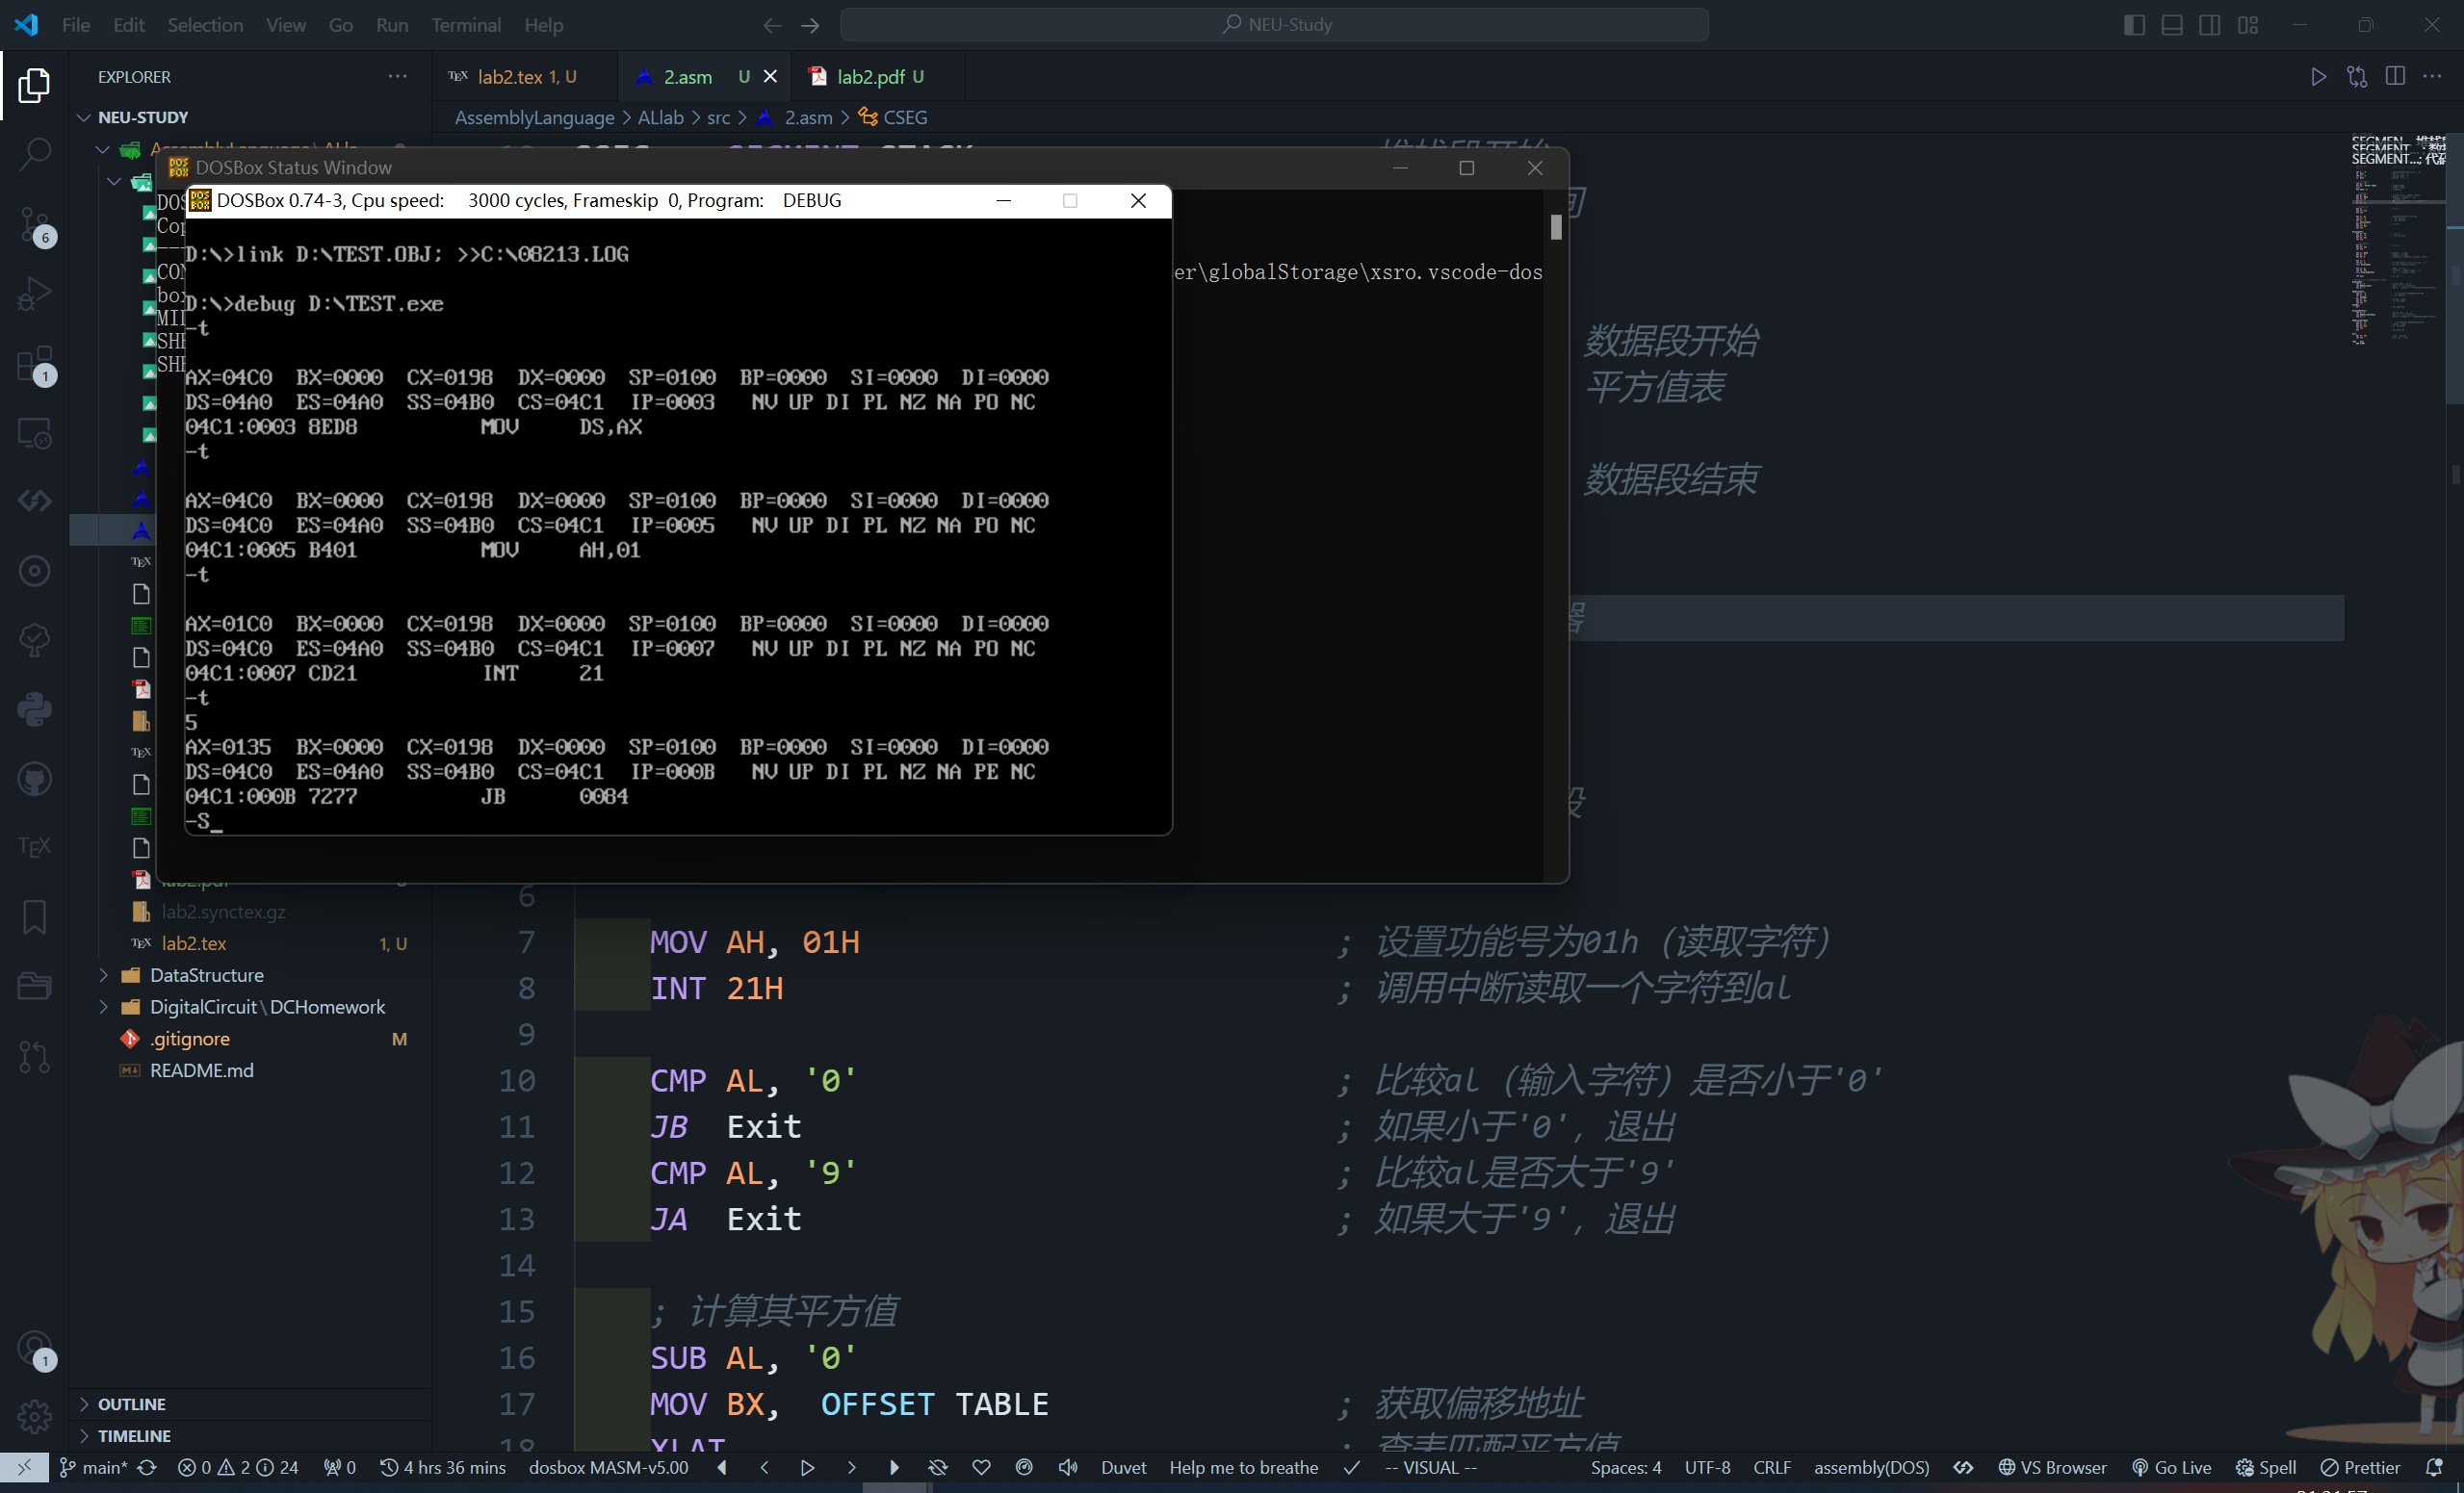
\includegraphics[width=1\textwidth]{image/AL_9.png}\end{center}
    \begin{center}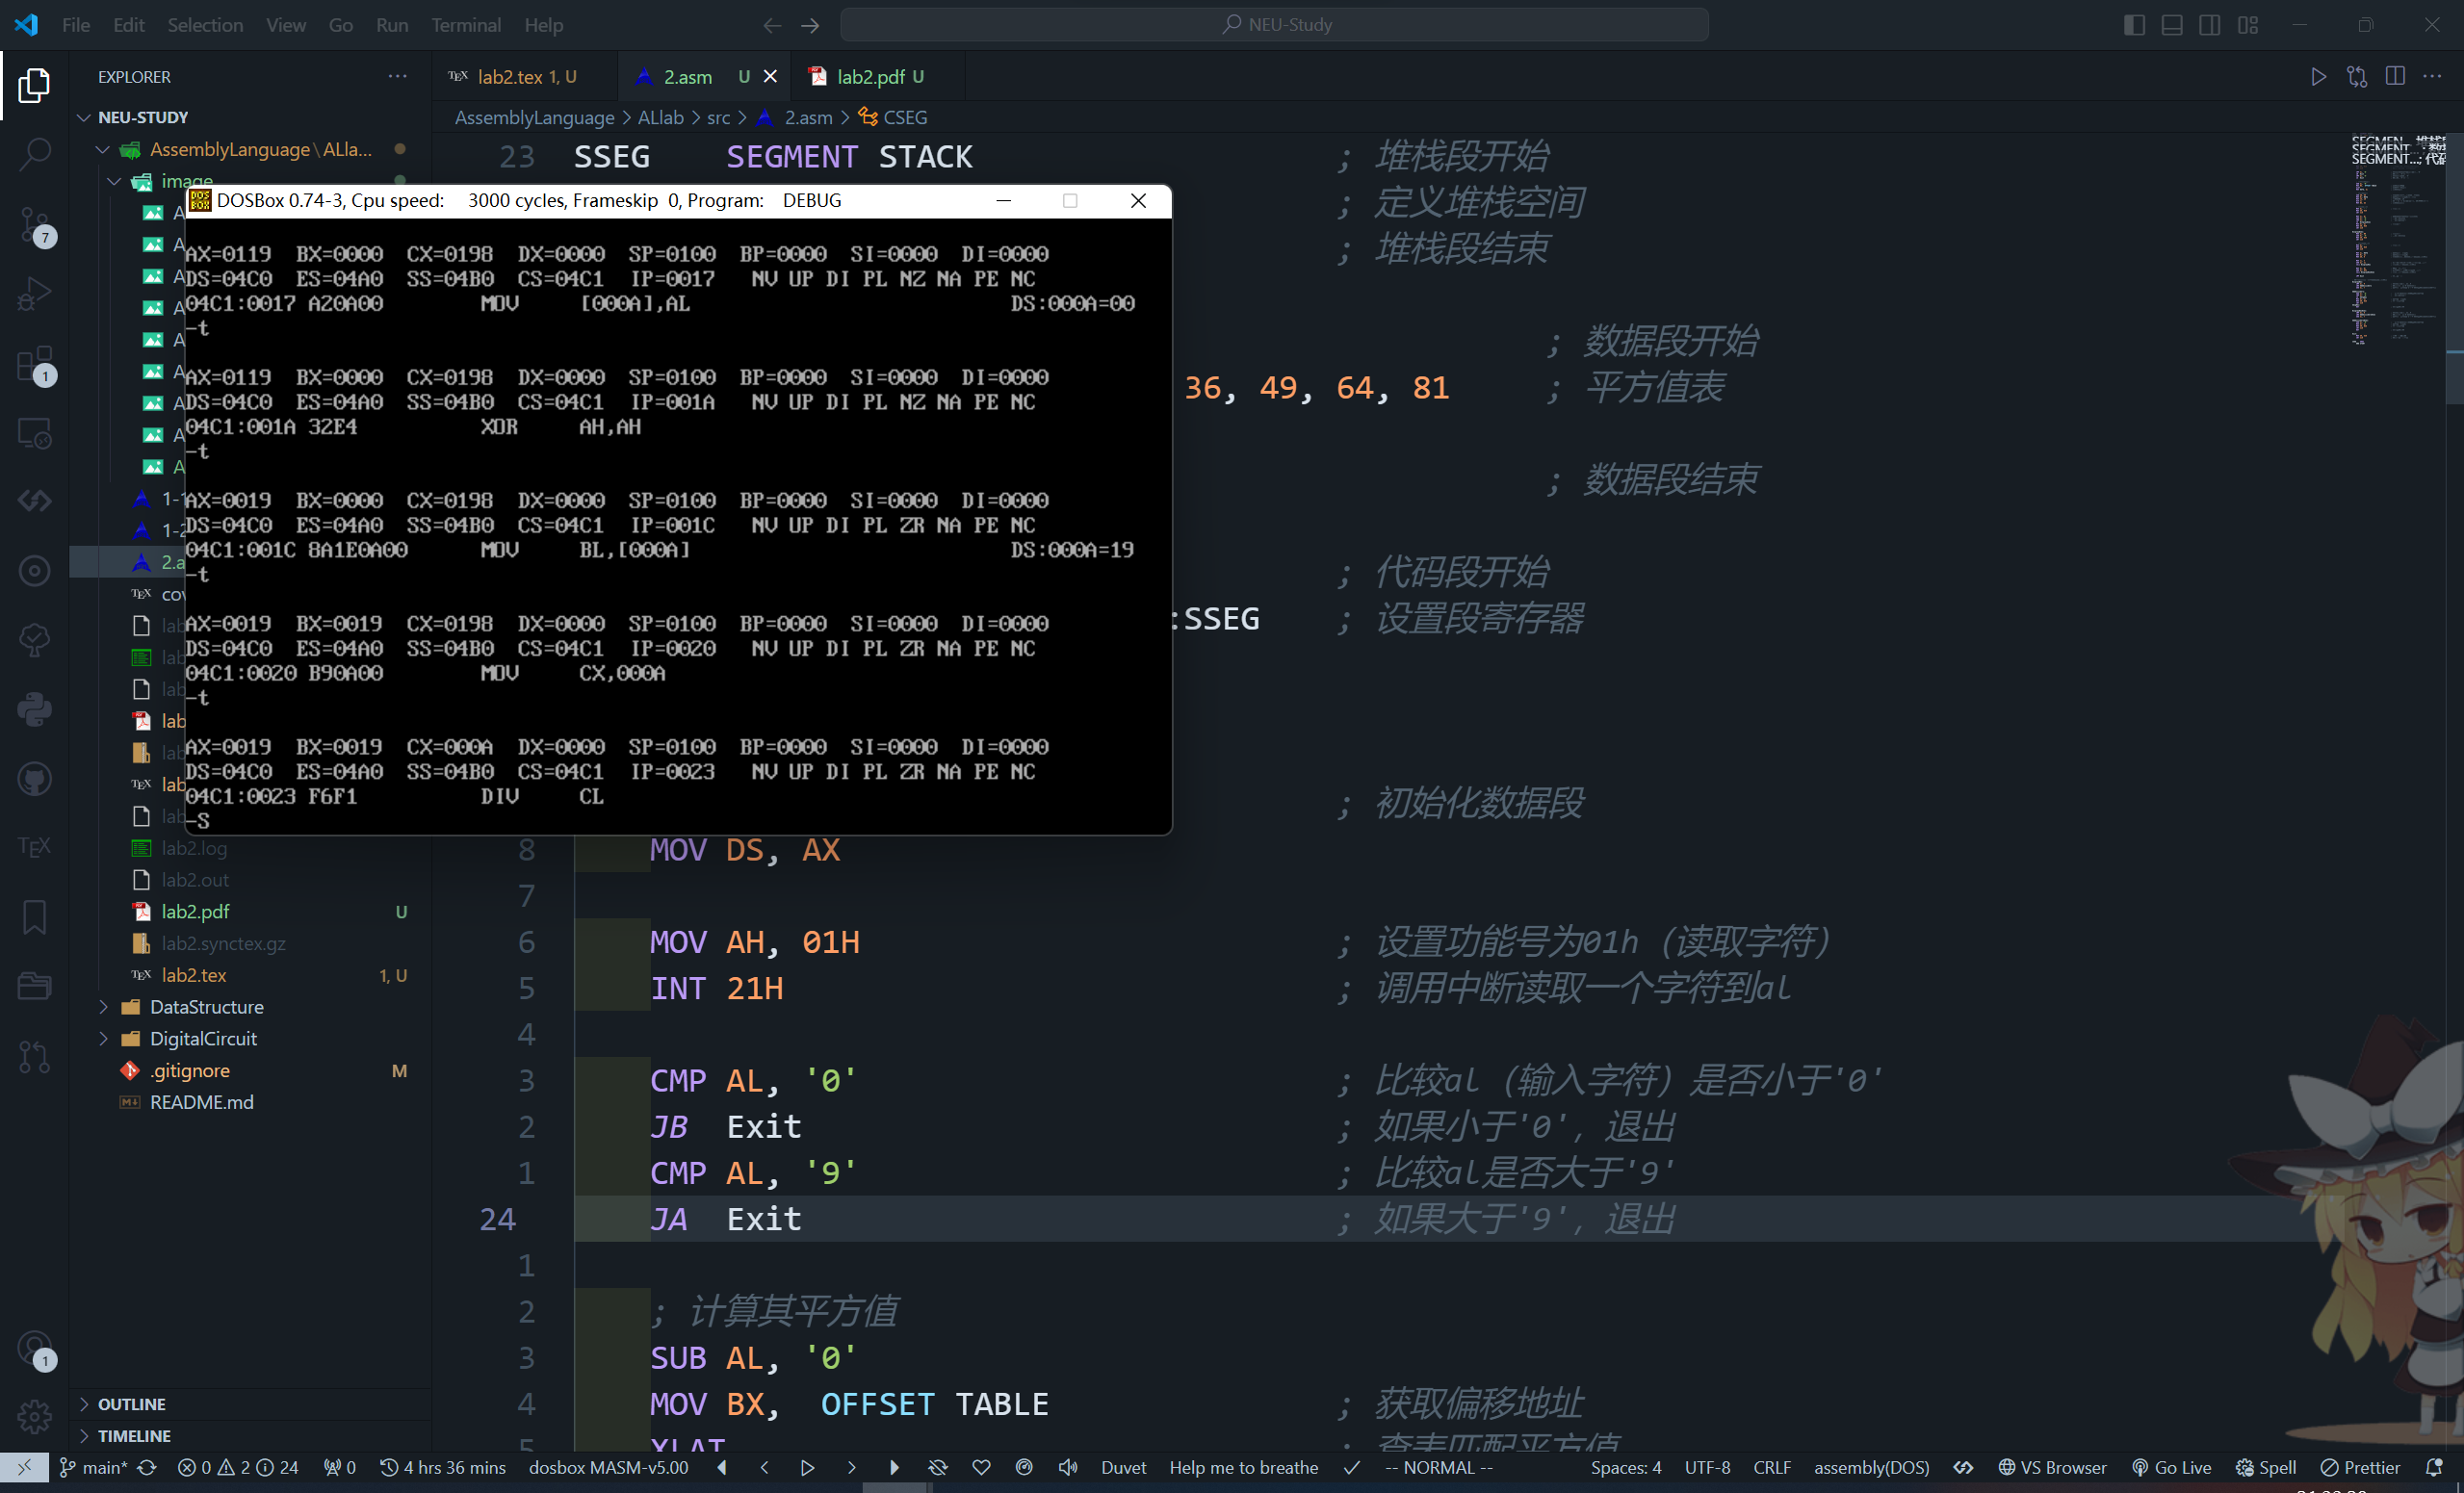
\includegraphics[width=1\textwidth]{image/AL_10.png}\end{center}
    \begin{center}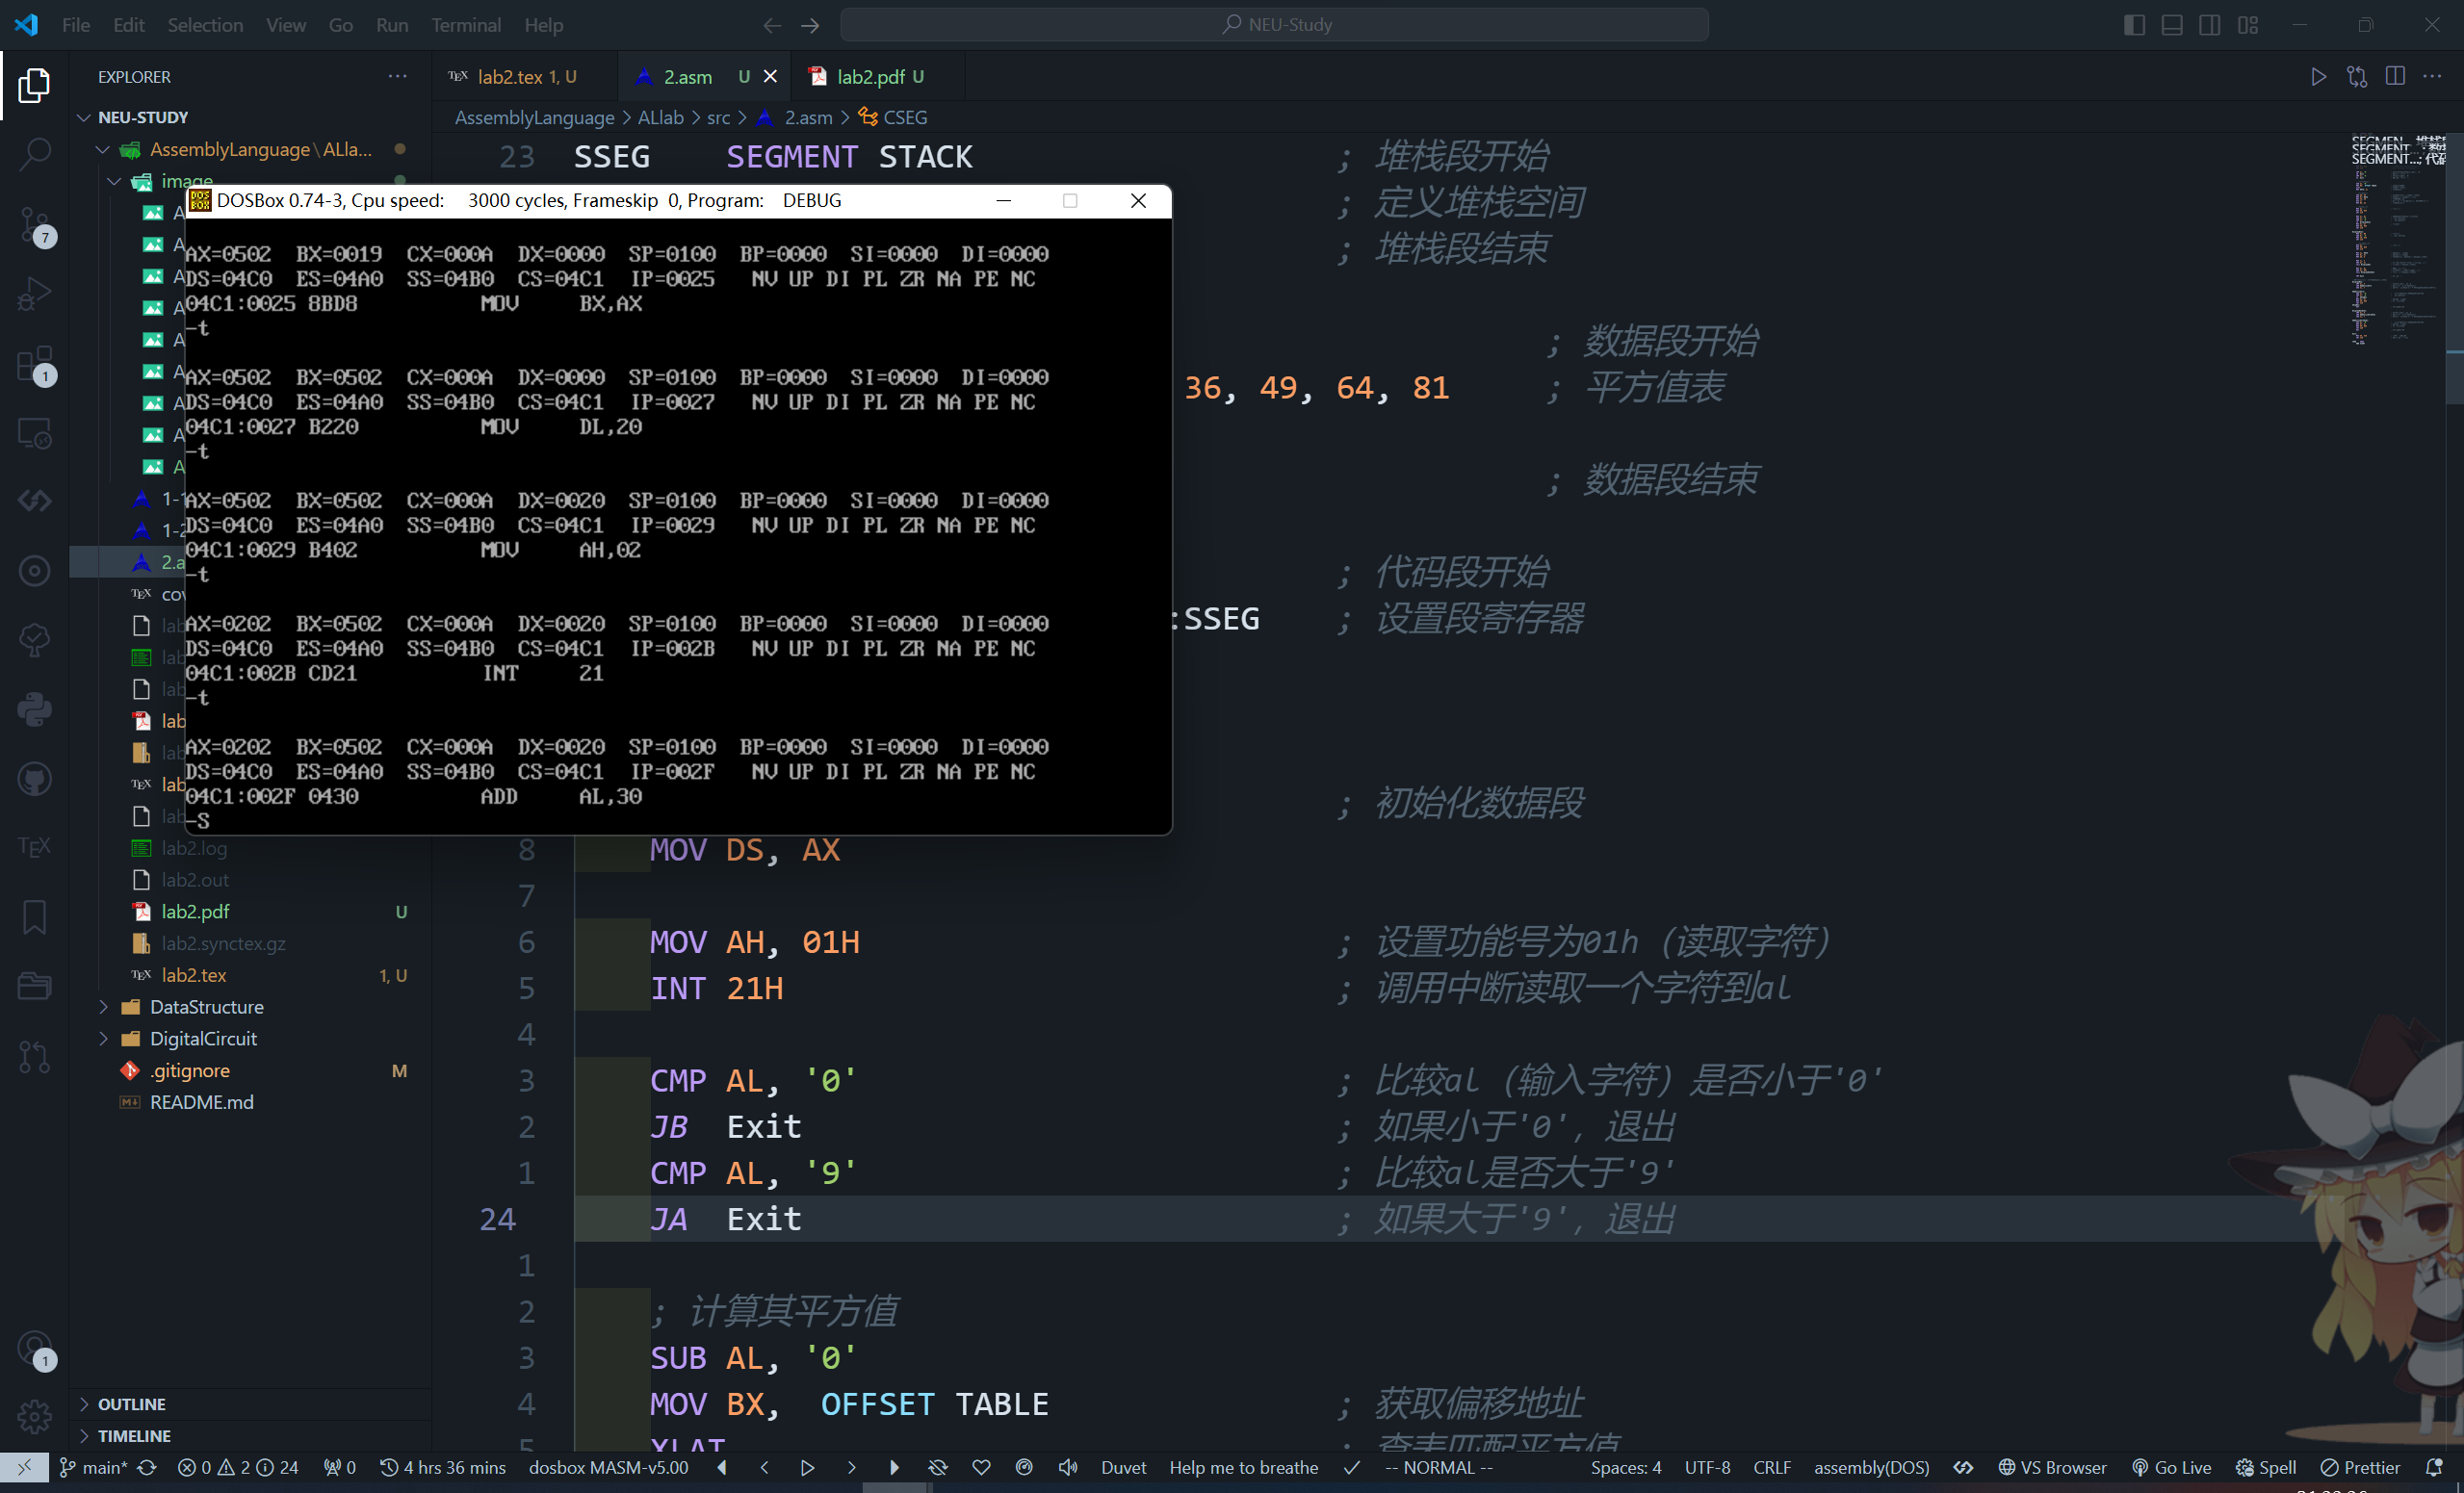
\includegraphics[width=1\textwidth]{image/AL_11.png}\end{center}
    \begin{center}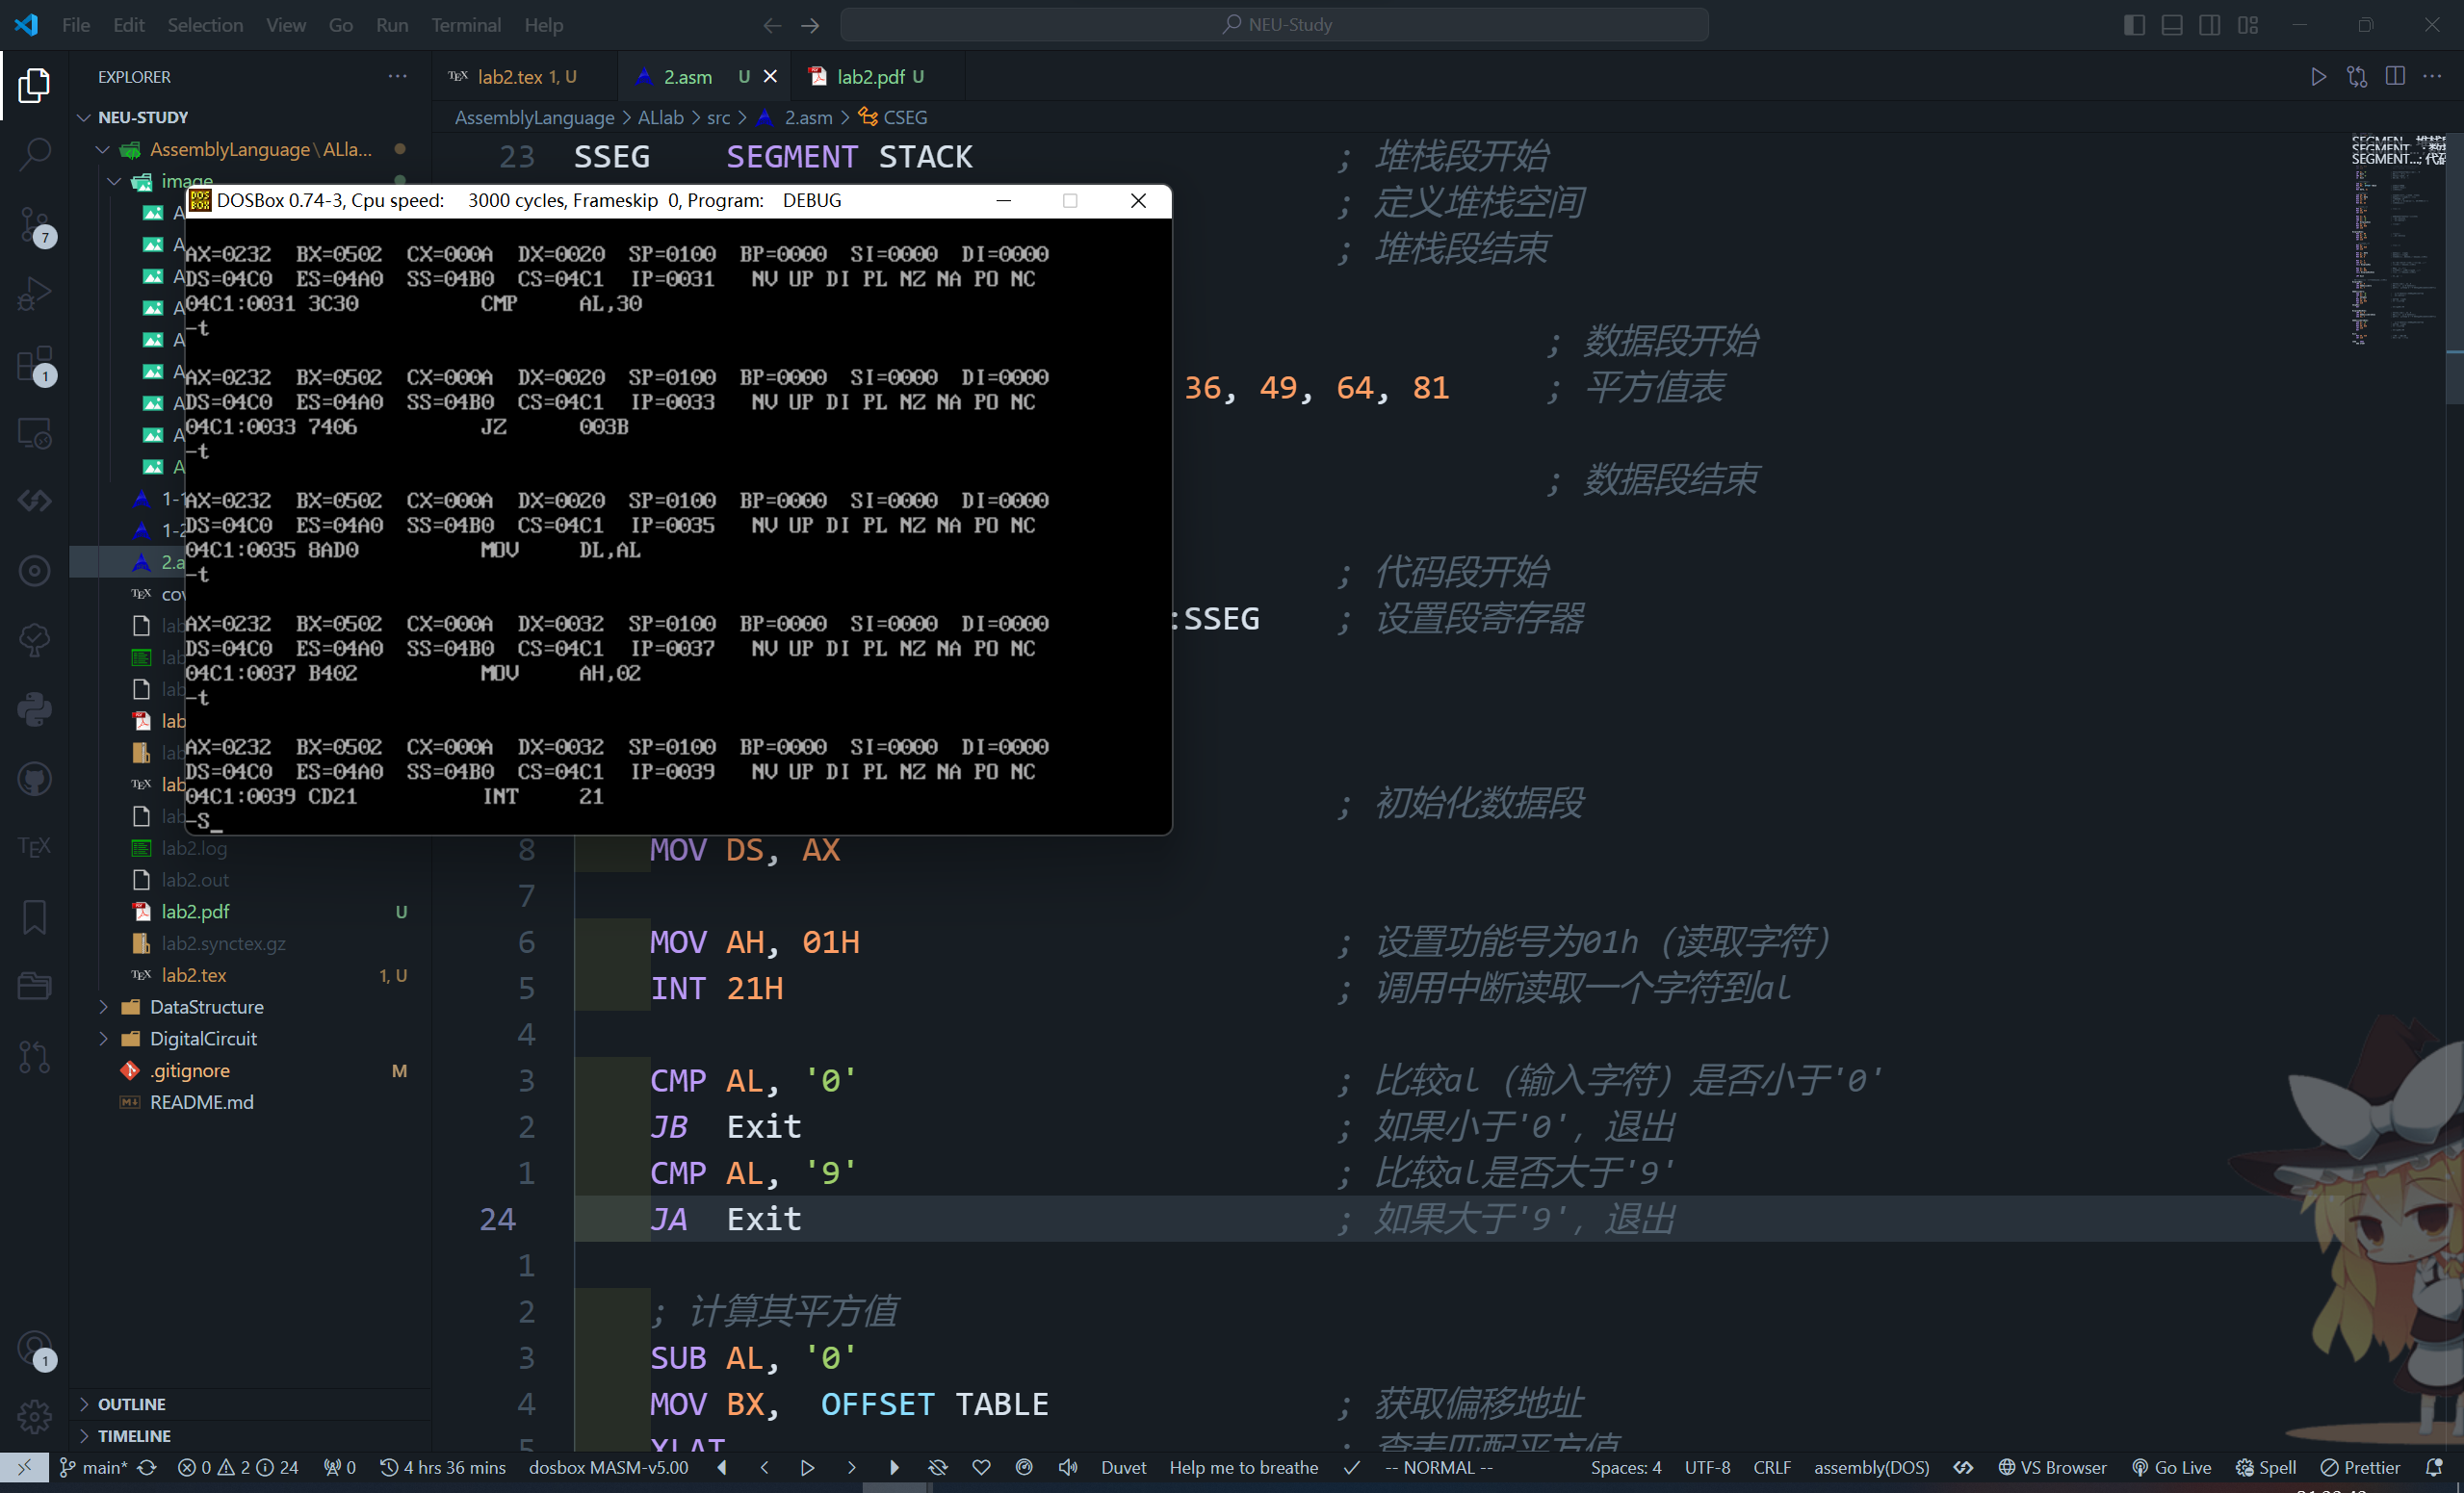
\includegraphics[width=1\textwidth]{image/AL_12.png}\end{center}
    \begin{center}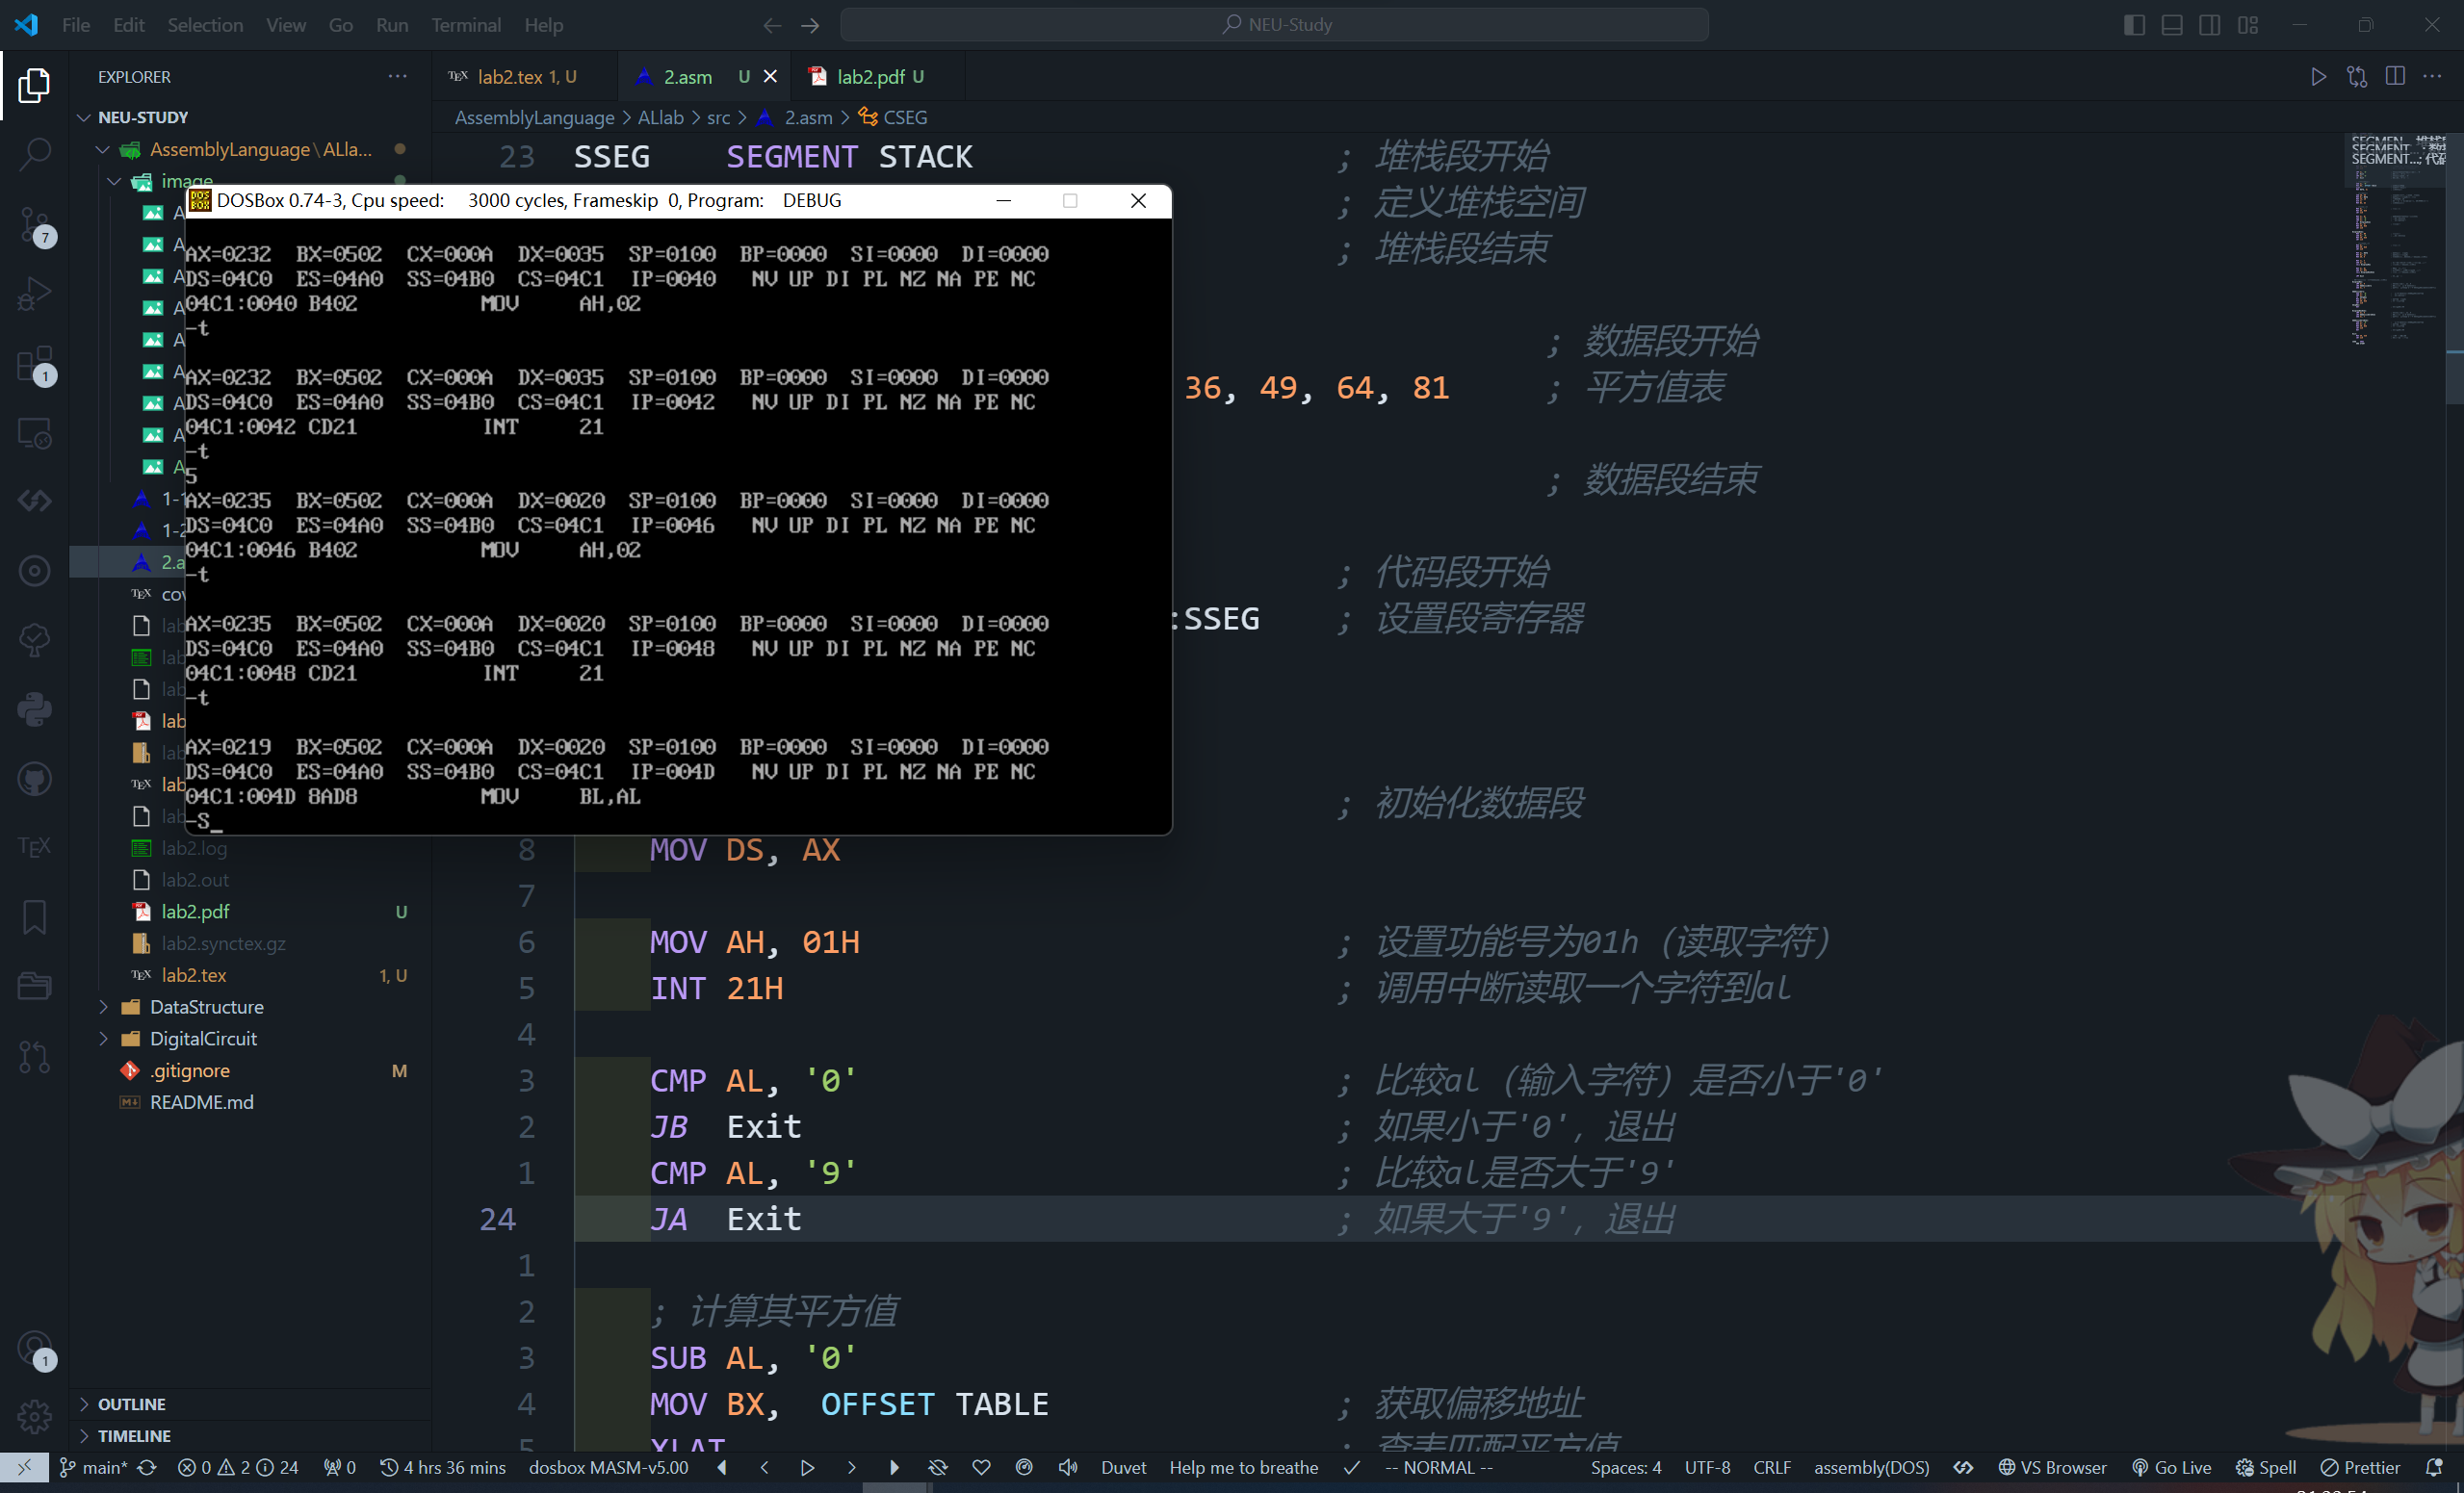
\includegraphics[width=1\textwidth]{image/AL_13.png}\end{center}
    \begin{center}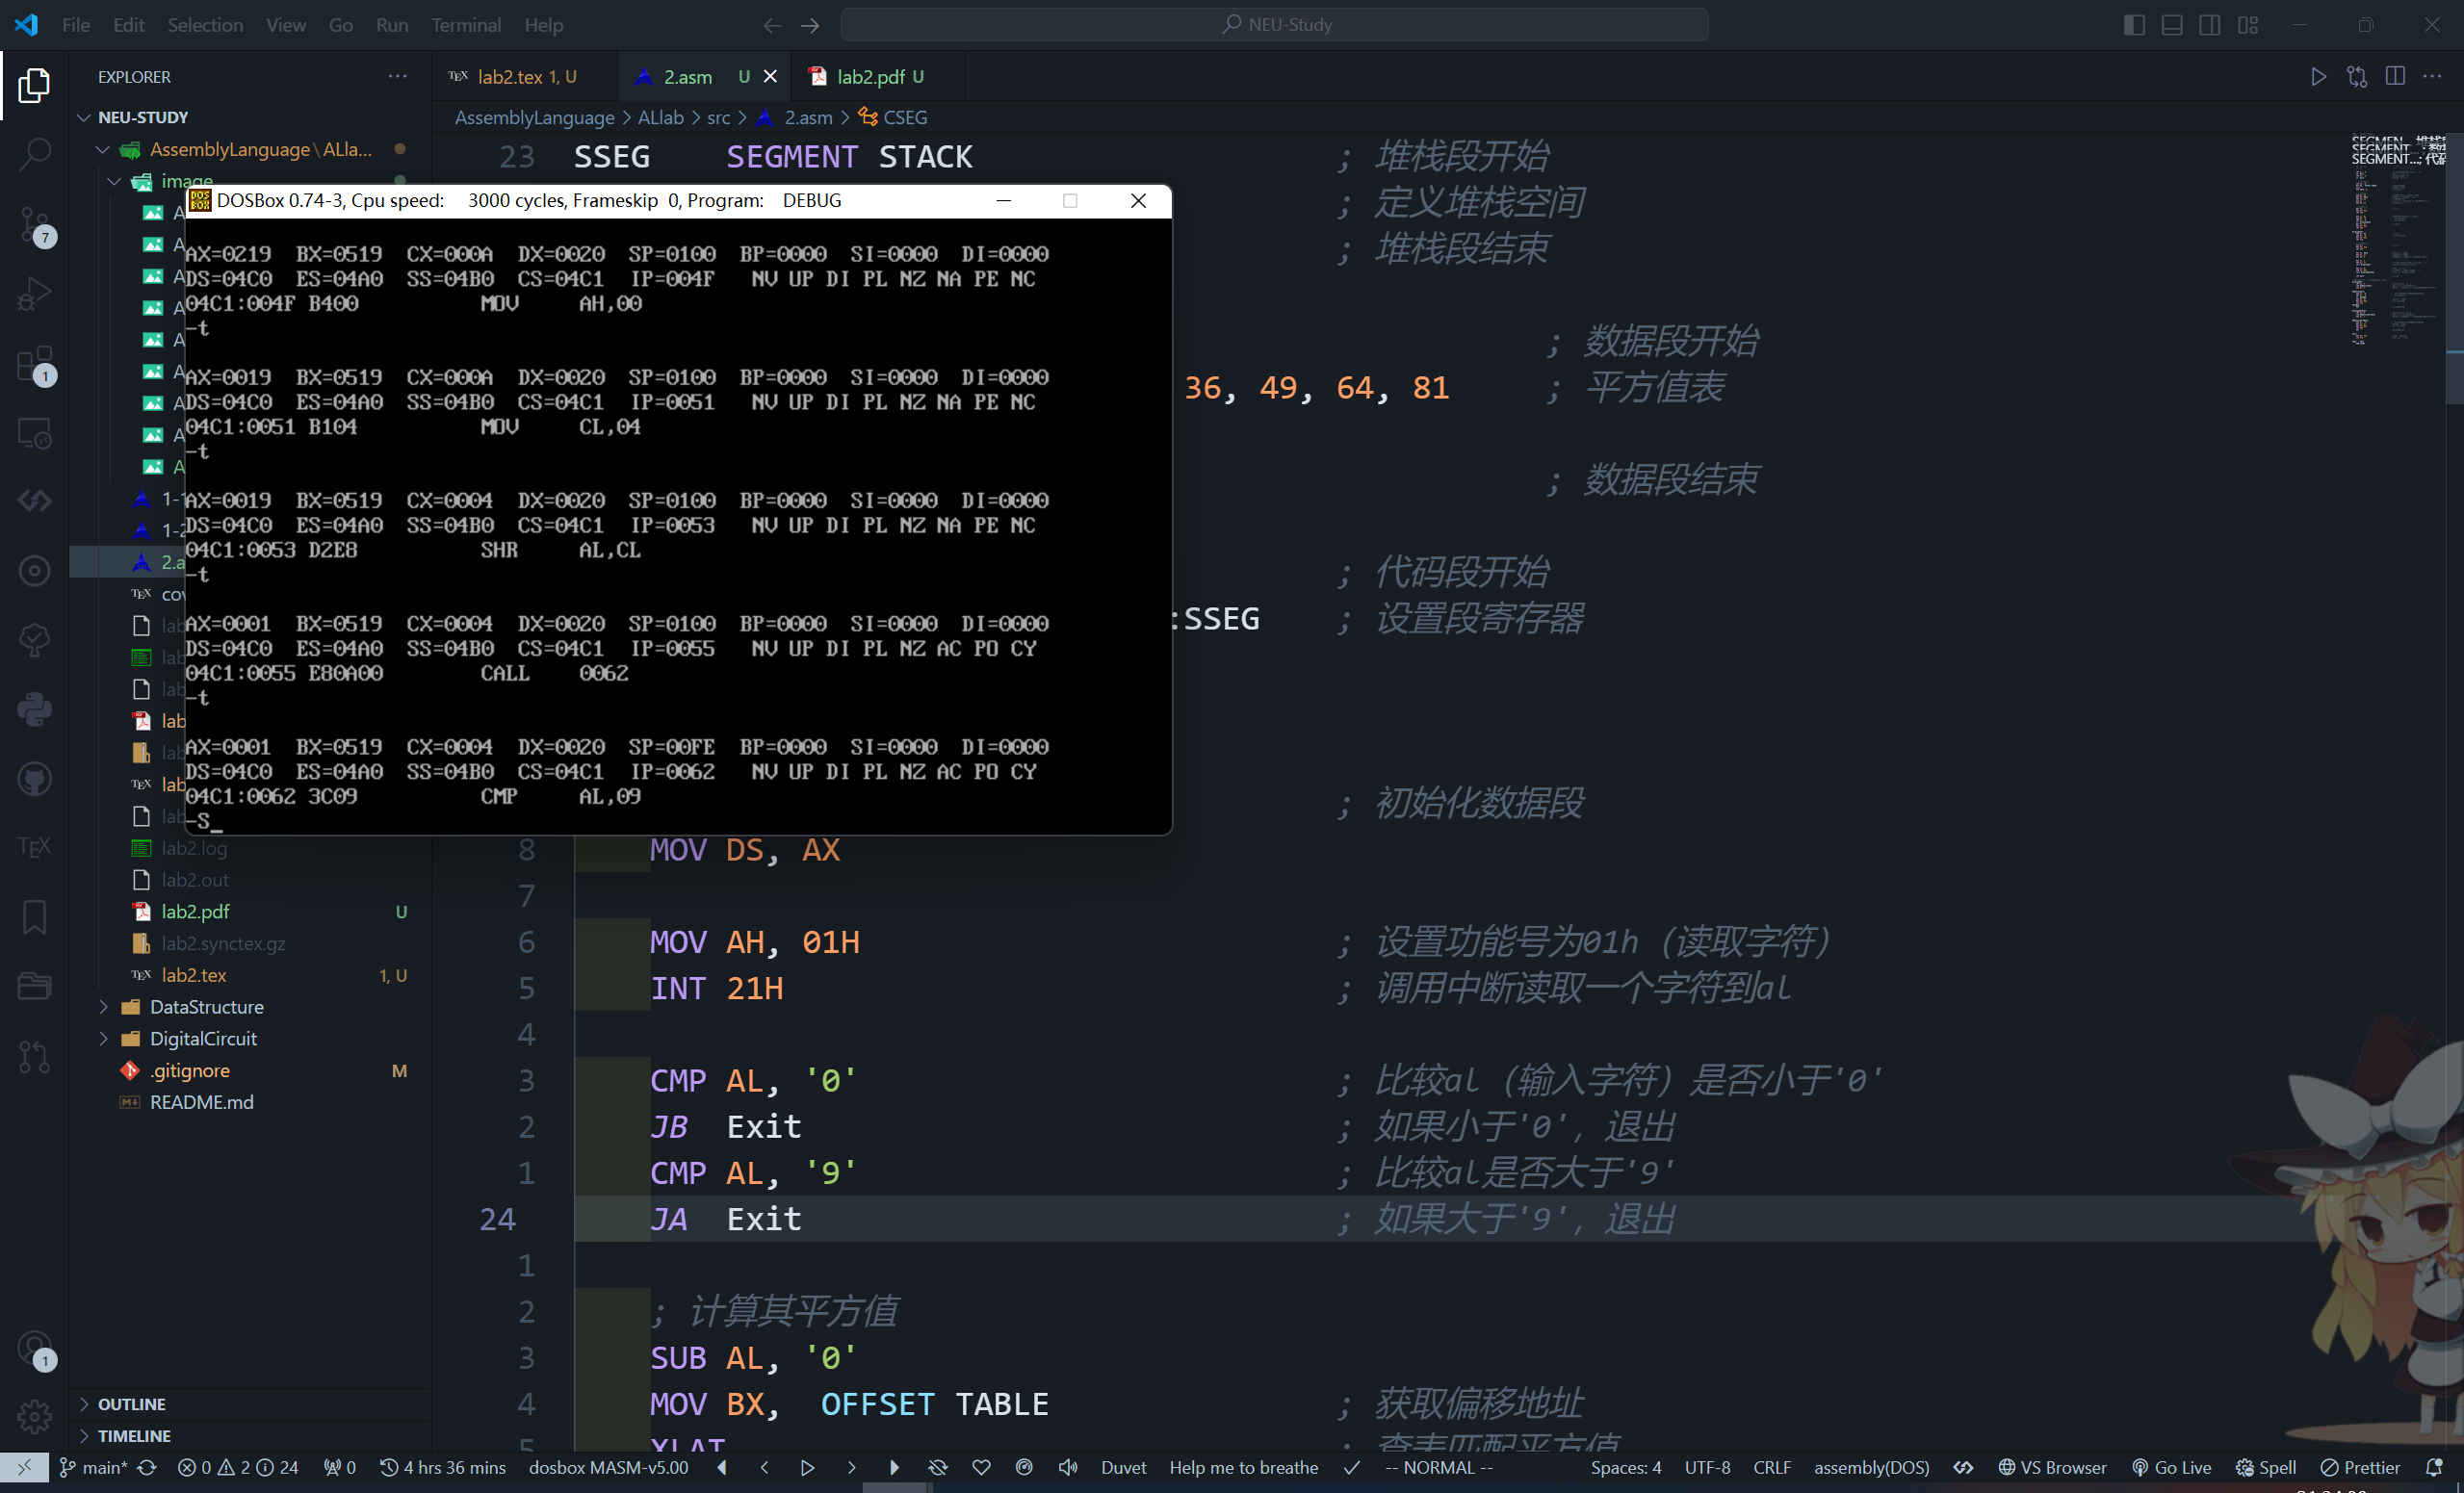
\includegraphics[width=1\textwidth]{image/AL_14.png}\end{center}
    \begin{center}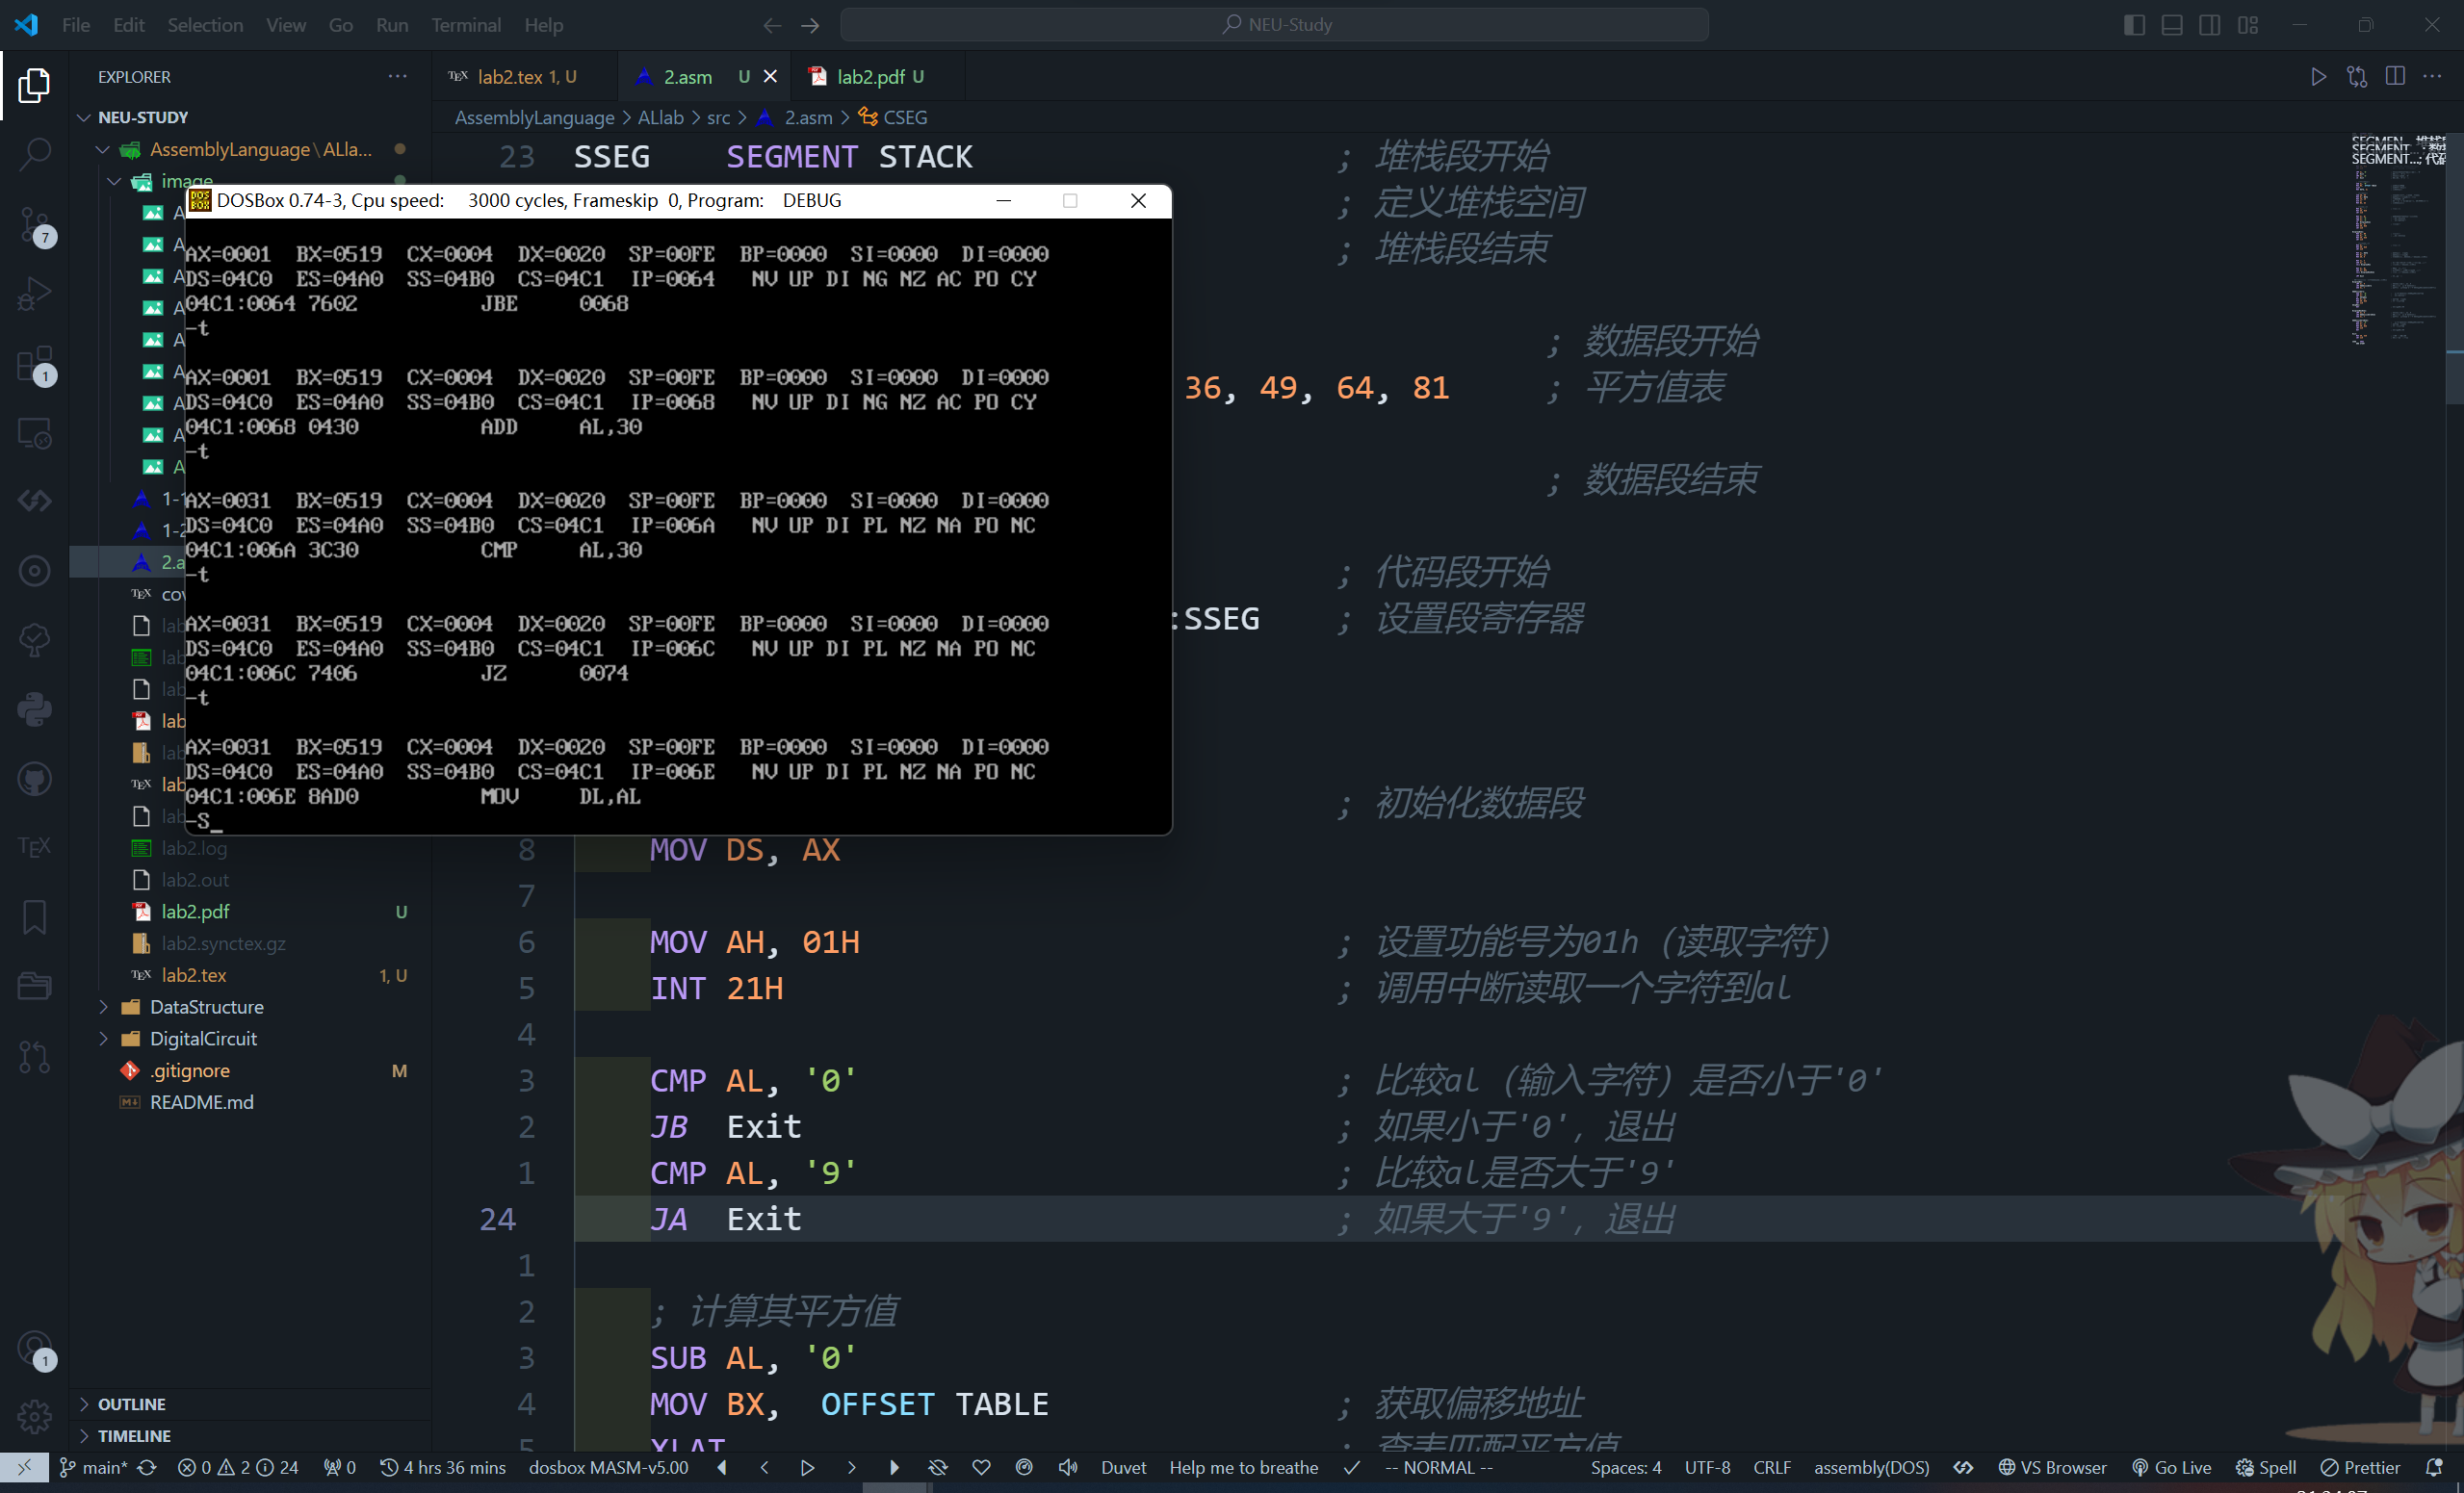
\includegraphics[width=1\textwidth]{image/AL_15.png}\end{center}
    \begin{center}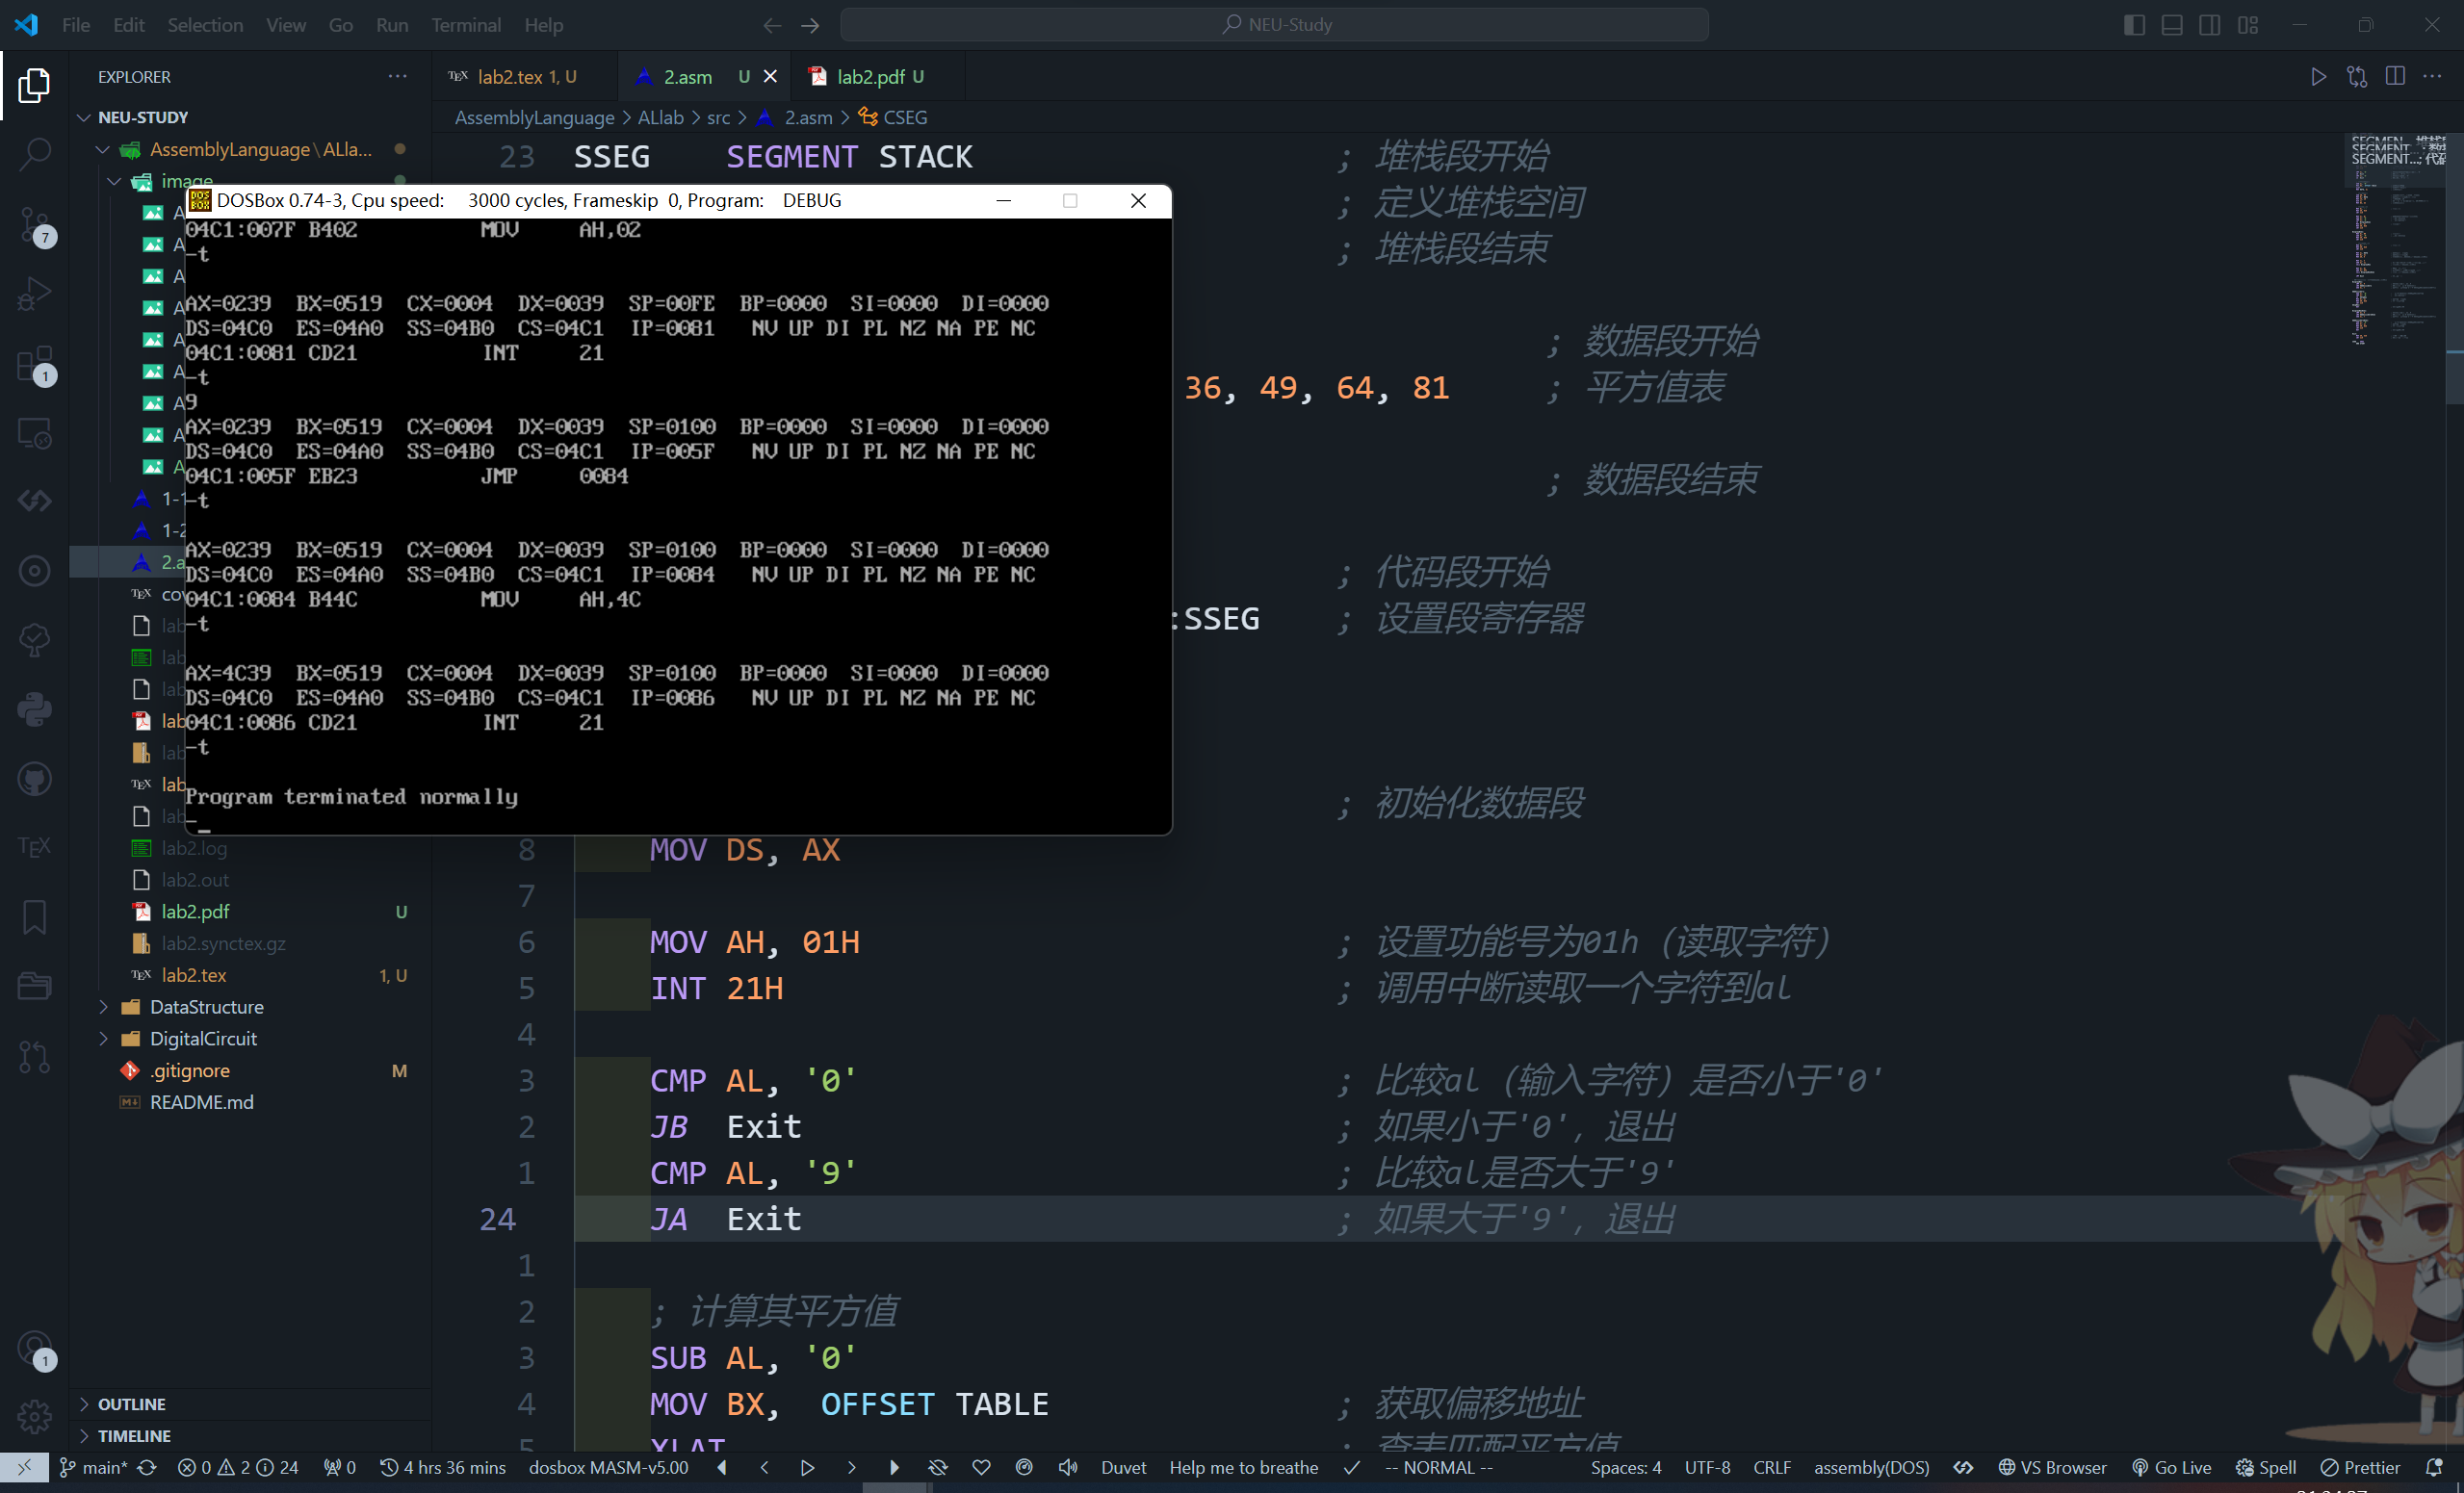
\includegraphics[width=1\textwidth]{image/AL_16.png}\end{center}

    \subsection{显示结果}
    1. 输入数字1，显示器上输出1的平方值1和1的十六进制表示1。
    \begin{center}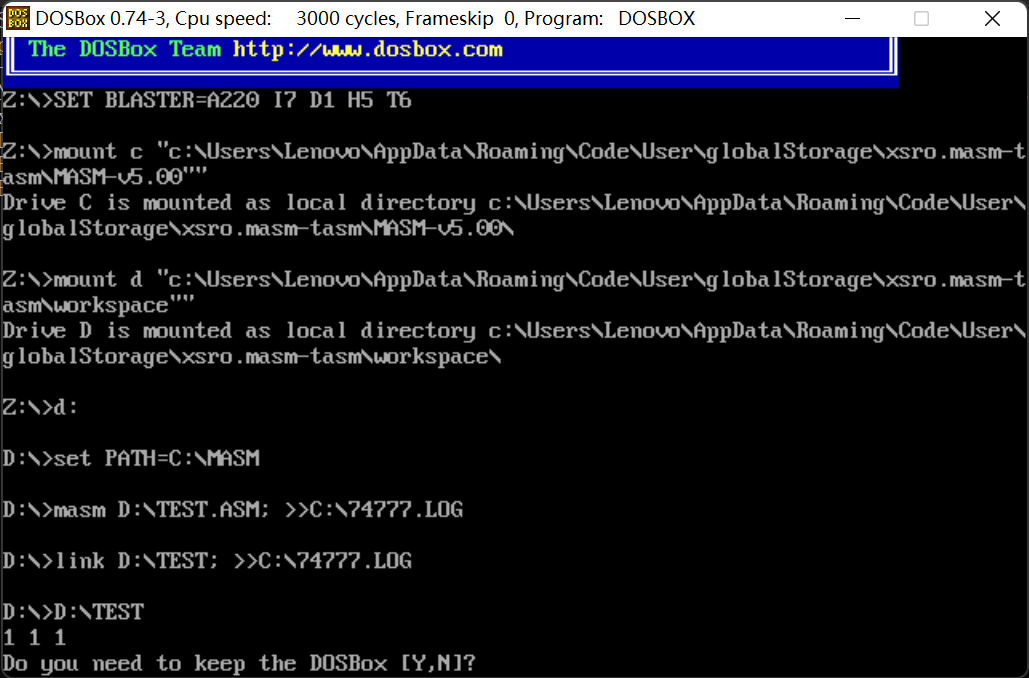
\includegraphics[width=1\textwidth]{image/AL_17.png}\end{center}
    2. 输入数字2，显示器上输出2的平方值4和2的十六进制表示4。
    \begin{center}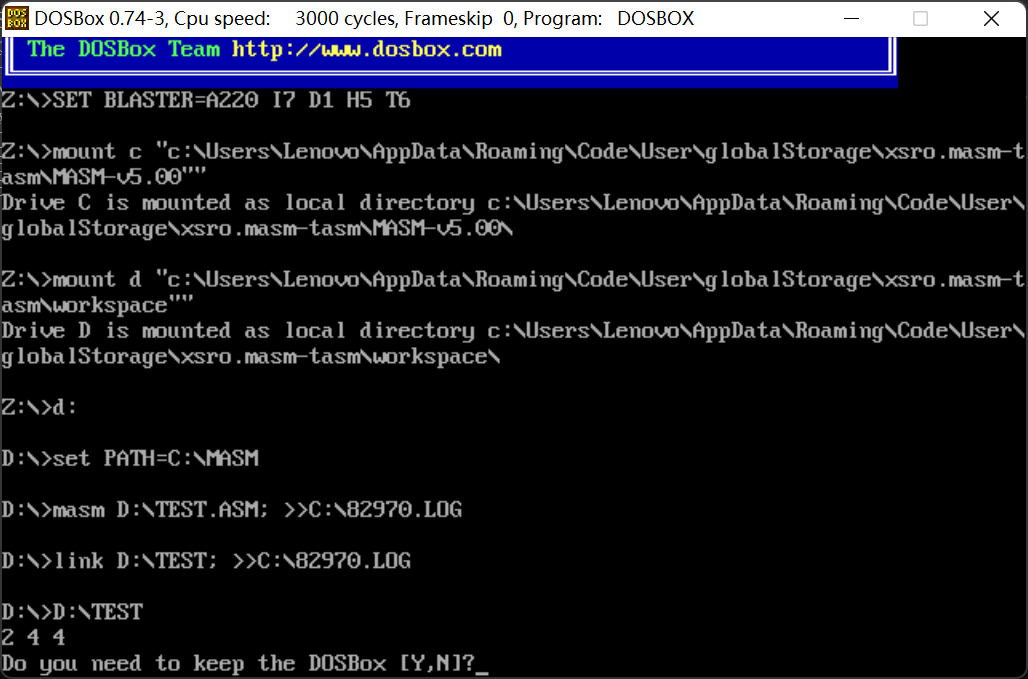
\includegraphics[width=1\textwidth]{image/AL_18.png}\end{center}
    3. 输入数字3，显示器上输出3的平方值9和3的十六进制表示9。
    \begin{center}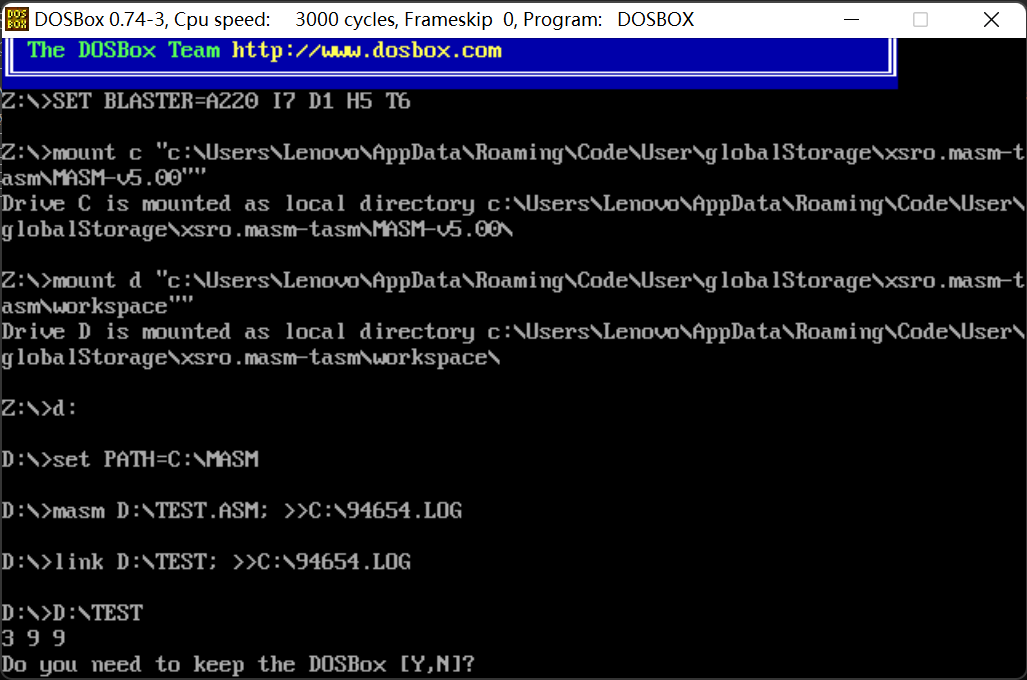
\includegraphics[width=1\textwidth]{image/AL_19.png}\end{center}
    4. 输入数字4，显示器上输出4的平方值16和4的十六进制表示10。
    \begin{center}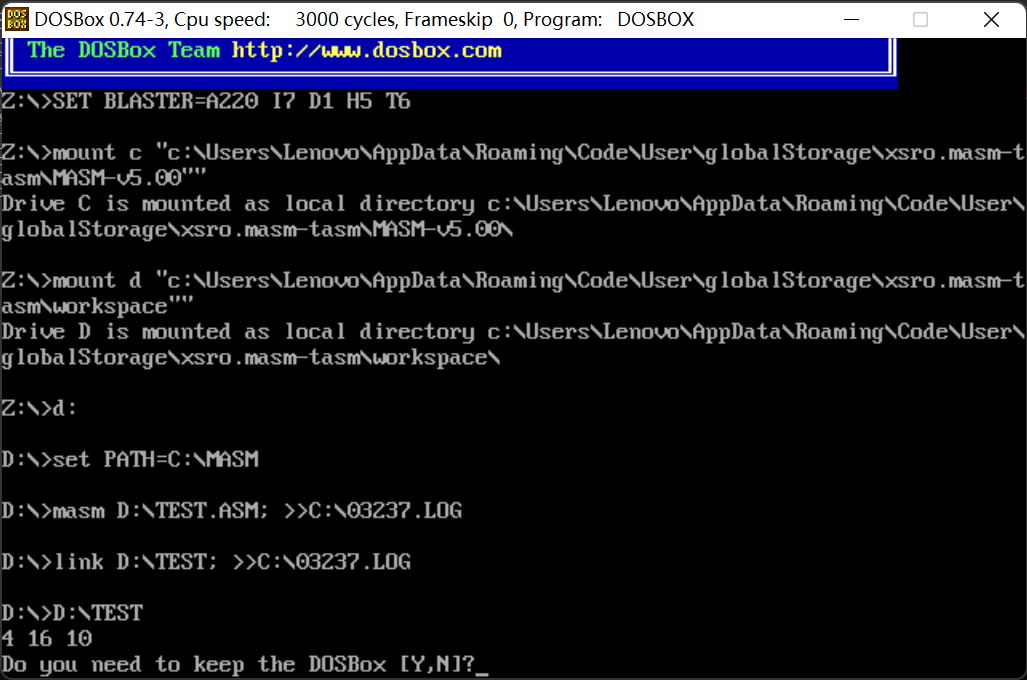
\includegraphics[width=1\textwidth]{image/AL_20.png}\end{center}
    5. 输入数字5，显示器上输出5的平方值25和5的十六进制表示19。
    \begin{center}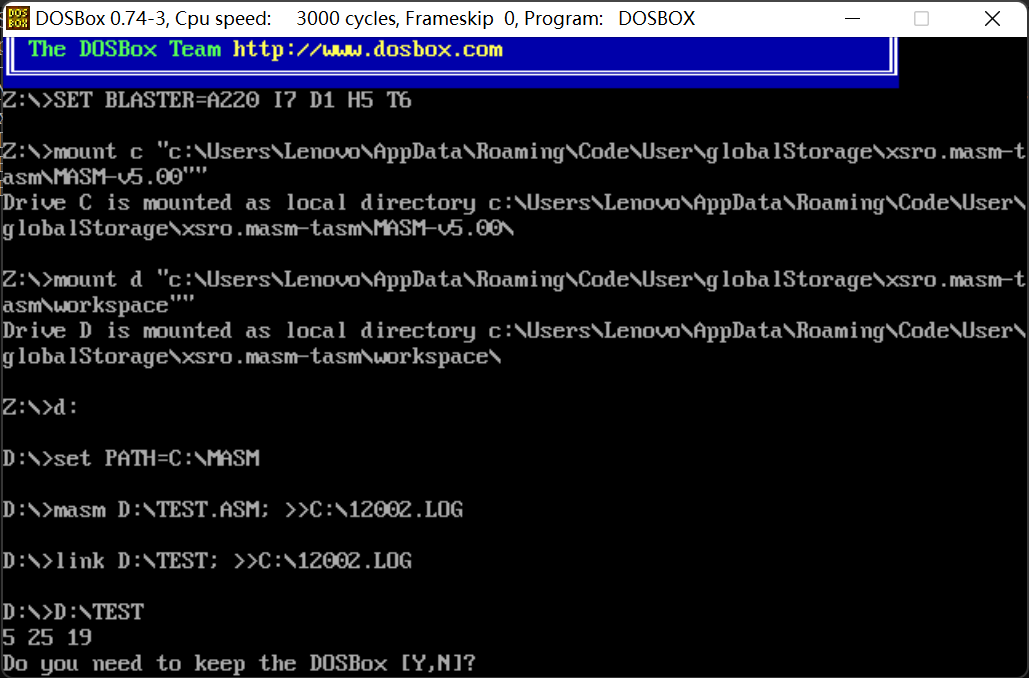
\includegraphics[width=1\textwidth]{image/AL_21.png}\end{center}
    6. 输入数字6，显示器上输出6的平方值36和6的十六进制表示24。
    \begin{center}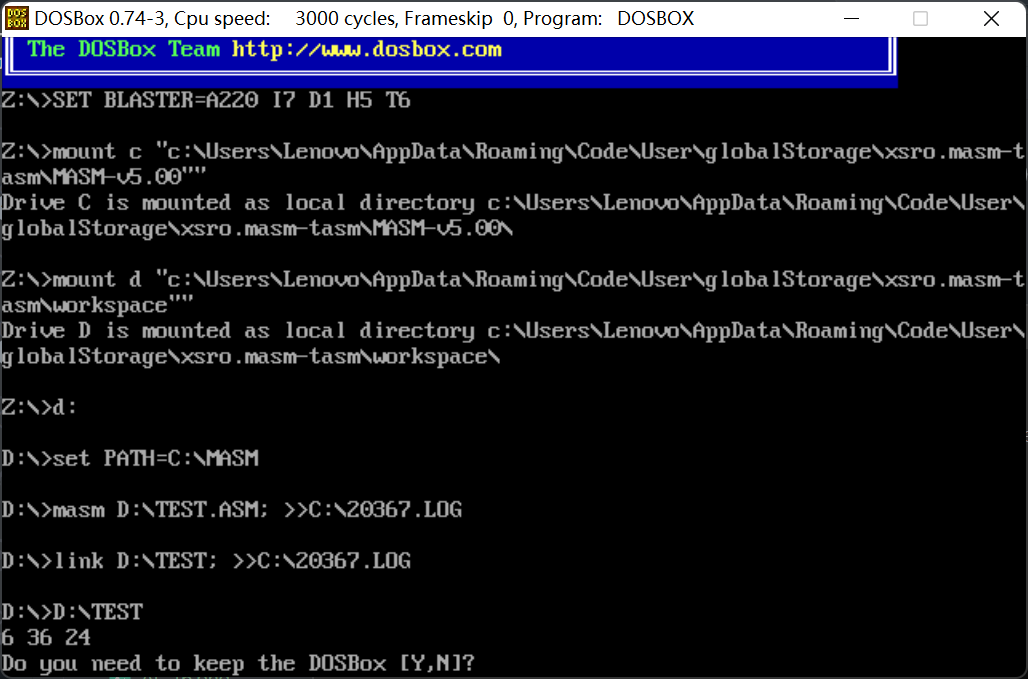
\includegraphics[width=1\textwidth]{image/AL_22.png}\end{center}
    7. 输入数字7，显示器上输出7的平方值49和7的十六进制表示31。
    \begin{center}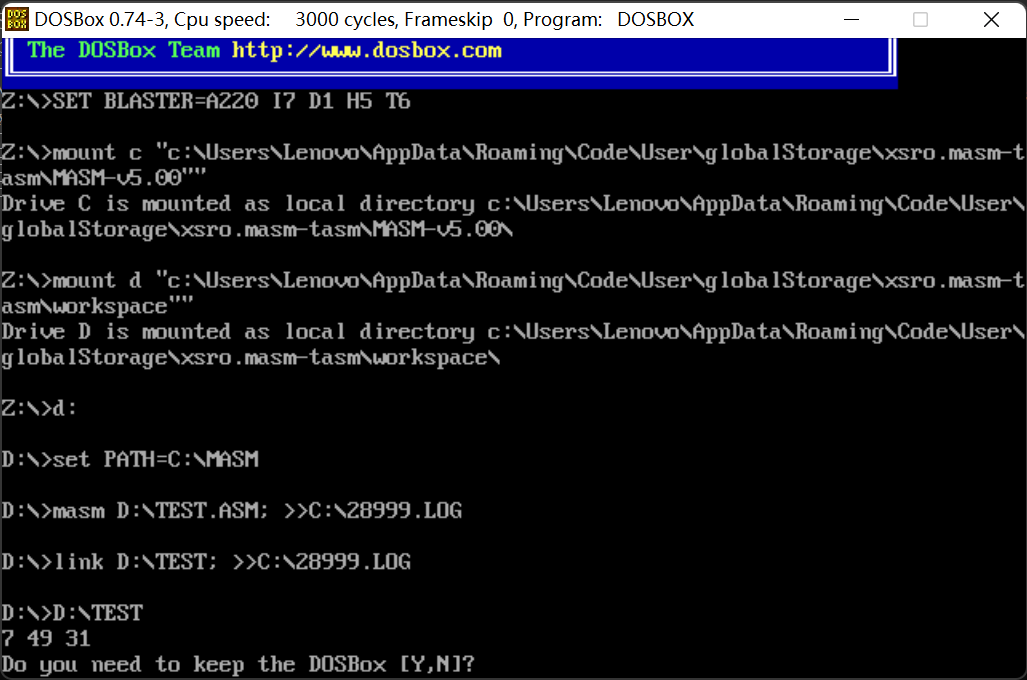
\includegraphics[width=1\textwidth]{image/AL_23.png}\end{center}
    8. 输入数字8，显示器上输出8的平方值64和8的十六进制表示40。
    \begin{center}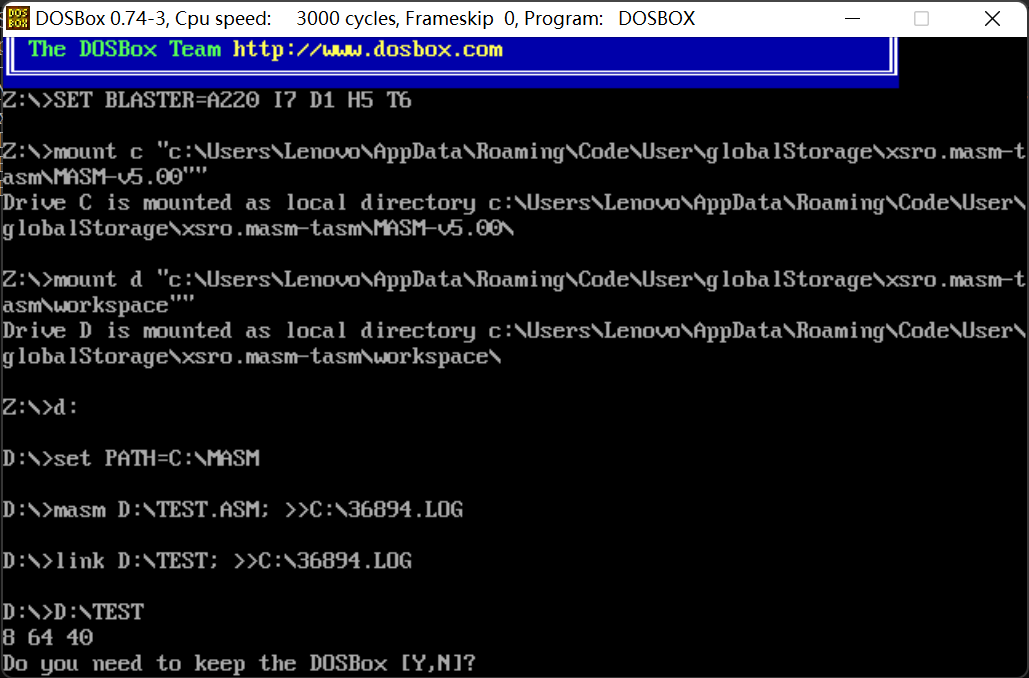
\includegraphics[width=1\textwidth]{image/AL_24.png}\end{center}
    9. 输入数字9，显示器上输出9的平方值81和9的十六进制表示51。
    \begin{center}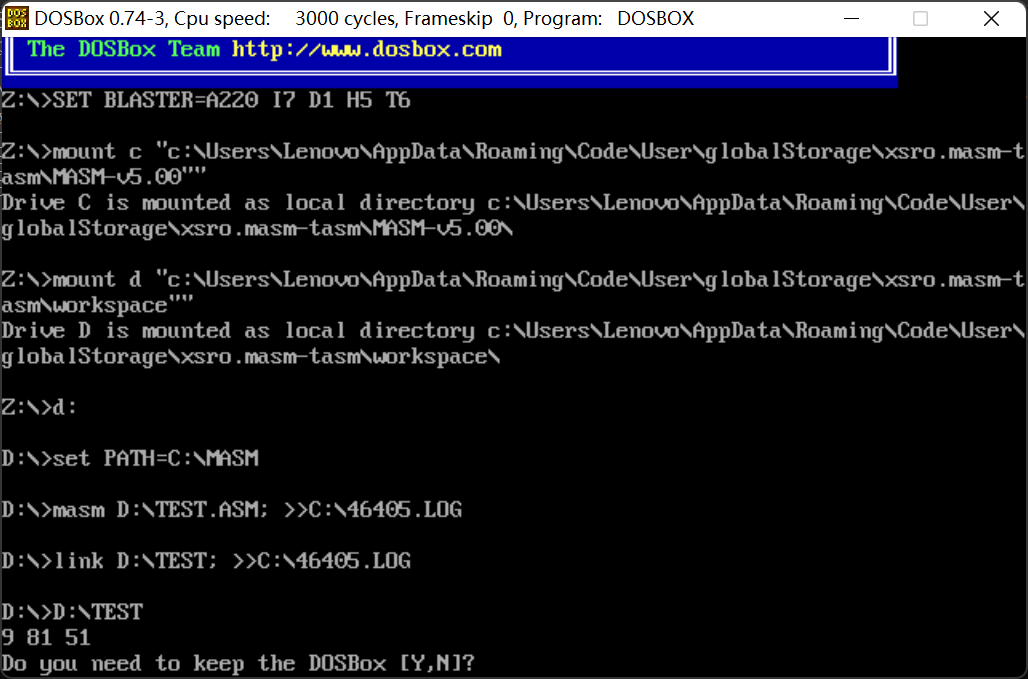
\includegraphics[width=1\textwidth]{image/AL_25.png}\end{center}

\section{心得体会}
通过完成这次汇编语言的实验，我深刻体会到了理论知识与实际操作之间的关系。在实验过程中，我不仅巩固了汇编语言的基础知识，还学习到了如何将理论应用到实际问题解决中。尤其是在进行数据转换和显示输出时，我更加深入地理解了汇编语言的强大和灵活性。

在实验过程中，我遇到了一些挑战，特别是在进行数据的十进制和十六进制转换时。最初，我对如何有效地利用查表方法进行转换感到困惑。但通过不断尝试和调试，我最终找到了解决问题的方法，这极大地提升了我的问题解决能力和编程技巧。

此外，这次实验也使我更加熟练地使用了调试工具，这在以后的编程学习和工作中将非常有用。总之，这次实验不仅提高了我的技术技能，也增强了我的自学能力和解决复杂问题的能力。
\begin{flushright}\begin{tabular}{rl}
    姓名: & 李俊洁\\
    班级: & 计算机2204 \\
    学号: & 20225443 \\
    课程: & 汇编语言程序设计 \\
    日期: & March 27, 2024 \\
    制作: & \LaTeX \\
    & 感谢您的批阅！
\end{tabular}\end{flushright}
\end{document}